\documentclass[manuscript, review, anonymous]{acmart}

\usepackage{booktabs} % For formal tables

\usepackage[ruled,vlined]{algorithm2e} % For algorithms
\renewcommand{\algorithmcfname}{ALGORITHM}
\SetAlFnt{\small}
\SetAlCapFnt{\small}
\SetAlCapNameFnt{\small}
\SetAlCapHSkip{0pt}
\IncMargin{-\parindent}

\usepackage{algorithmic}
\usepackage{graphicx}
\usepackage{textcomp}
\usepackage{xcolor}
\usepackage{subcaption}

\newcommand{\ra}[1]{\renewcommand{\arraystretch}{#1}}
\usepackage{tabularx}
\newcolumntype{L}[1]{>{\hsize=#1\hsize\raggedright\arraybackslash}X}%

%\let\comment\undefined      % neutralize \comment command
\usepackage{comment}
\usepackage[markup=underlined]{changes}
\definechangesauthor[color=orange]{ES}
\newcommand{\ES}[1]{\added[id=ES]{#1}}
\definecolor{darkgreen}{rgb}{0.29, 0.40, 0.13}
\definechangesauthor[color=darkgreen]{KT}
\newcommand{\KT}[1]{\added[id=KT]{#1}}
\definechangesauthor[color=blue]{SL}
\newcommand{\SL}[1]{\added[id=SL]{#1}}

% Metadata Information
%\acmJournal{THRI}
%\acmVolume{9}
%\acmNumber{4}
%\acmArticle{39}
%\acmYear{2010}
%\acmMonth{3}
%\copyrightyear{2009}
%\acmArticleSeq{9}

% Copyright
%\setcopyright{acmcopyright}
%\setcopyright{acmlicensed}
%\setcopyright{rightsretained}
%\setcopyright{usgov}
%\setcopyright{usgovmixed}
%\setcopyright{cagov}
%\setcopyright{cagovmixed}

%\setcopyright{acmcopyright}
%\copyrightyear{2018}
%\acmYear{2018}
%\acmDOI{10.1145/1122445.1122456}

%% These commands are for a PROCEEDINGS abstract or paper.
%\acmConference[HRI '20]{ }{ }{Woodstock, NY}
%\acmBooktitle{Woodstock '18: ACM Symposium on Neural Gaze Detection,
%	June 03--05, 2018, Woodstock, NY}
%\acmPrice{15.00}
%\acmISBN{978-1-4503-9999-9/18/06}

% DOI
%\acmDOI{0000001.0000001}

% Paper history
%\received{February 2007}
%\received[revised]{March 2009}
%\received[accepted]{June 2009}

\usepackage{xspace}
\newcommand{\woz}{WoZ++\xspace}

% Document starts
\begin{document}
% Title portion. Note the short title for running heads
    \title{Wizard-of-Oz++: A Participatory Path to Autonomy}

\author{Redacted for review}
\email{************}
\affiliation{%
  \institution{********}
  \state{****}
  }
  
  \author{Redacted for review}
\email{************}
\affiliation{%
  \institution{********}
  \state{****}
  }
  
  \author{Redacted for review}
\email{************}
\affiliation{%
  \institution{********}
  \state{****}
  }
%    \author{Emmanuel Senft}
%    \affiliation{%
%        \institution{Centre for Robotics and Neural Systems, Univervsity of Plymouth}
%        \city{Plymouth}
%        \country{UK}}
%    \author{S\'everin Lemaignan}
%    \affiliation{%
%        \institution{Bristol Robotics Lab, University of the West of England}
%        \city{Bristol}
%        \country{UK}
%    }
%   \author{Paul E. Baxter}
%    \affiliation{%
%        \institution{Lincoln Centre for Autonomous Systems, University of Lincoln}
%        \city{Lincoln}
%        \country{UK}}
%    \author{Tony Belpaeme}
%    \affiliation{%
%        \institution{Centre for Robotics and Neural Systems, University of Plymouth, UK - IDLab - imec, Ghent University, BE}
%    }


\begin{abstract}

    This paper presents an evolution of the classical Wizard-of-Oz (WoZ) control
    methodology, that maintains key properties of WoZ (e.g. human supervision at
    runtime) while using machine learning to transparently learn the wizard's
    latent policy.
    This paper proposes to transform the \emph{wizard}, controlling the robot, into a 
    \emph{teacher} actively transmitting knowledge to the robot; thus resulting 
    in a robot becoming progressively autonomous.
    %Classical `offline' learning has been applied successfully in HRI (for
    %example by using Learning from Demonstration) but still possesses serious
    %constraints (e.g. rigidity and discretisation of the learning process,
    %continuous requirement of engineering expertise and ``black box'' learning).
    Our methodology, \woz, avoids classical pitfalls of offline learning
    (e.g. rigidity and discretisation of the learning process,
    the requirement for engineering expertise and ``black box'' learning)
    by fully embedding the
    robot learning process into the target interaction: the robot learns by being 
    taught by a human
    as it interacts in the real world.  We support our approach by analysing
    two ecologically valid case studies where this methodology was deployed: 
    teaching a robot to support children in an educative game and teaching a robot to support a long-term exercise programme.
    Results from these studies showed that these robots could learn  
    satisfactory autonomous social policies in the real world in very little time, even in 
    high-dimensional environments and could learn to use people's personality traits in their policies.%\ES{would that be correct?} %\KT{I can't give you any evidence at this point that I learned `very quickly', my case study probably more about the complexity of combining static/personality data with the dynamic task performance than the speed of going autonomous!}
    %(in one case, 200+ input dimensions; 600+ discrete actions), 
    %the robot learns remarkably quickly a
    %satisfactory autonomous policy, that includes precise action timing and
    %social elements.  Full details of the study as well as the source code are
    %available online.

\end{abstract}


%
% The code below should be generated by the tool at
% http://dl.acm.org/ccs.cfm
% Please copy and paste the code instead of the example below.
%

\begin{CCSXML}
    <ccs2012>
    <concept>
    <concept_id>10010520.10010553.10010554.10010557</concept_id>
    <concept_desc>Computer systems organization~Robotic autonomy</concept_desc>
    <concept_significance>500</concept_significance>
    </concept>
    <concept>
    <concept_id>10003120.10003121</concept_id>
    <concept_desc>Human-centered computing~Human computer interaction (HCI)</concept_desc>
    <concept_significance>300</concept_significance>
    </concept>
    <concept>
    <concept_id>10010147.10010178.10010187.10010194</concept_id>
    <concept_desc>Computing methodologies~Cognitive robotics</concept_desc>
    <concept_significance>300</concept_significance>
    </concept>
    </ccs2012>
\end{CCSXML}

\ccsdesc[500]{Computer systems organization~Robotic autonomy}
\ccsdesc[300]{Human-centered computing~Human computer interaction (HCI)}
\ccsdesc[300]{Computing methodologies~Cognitive robotics}


%
% End generated code
%

\keywords{Human-Robot Interaction, Progressive Autonomy, Robot Learning, Wizard of Oz, Interactive Machine Learning, Supervised Autonomy}

\maketitle

% The default list of authors is too long for headers.
%	\renewcommand{\shortauthors}{E. Senft, et al.}
%\ES{wizard vs teacher?}

\section{Introduction}

The field of social Human-Robot Interactions (HRI) covers a large range of
applications \cite{goodrich2007human}, with robots often interacting with
vulnerable populations, such as young children \cite{belpaeme2018social}, the
elderly \cite{wada2005psychological}, people requiring healthcare
\cite{dautenhahn1999robots} or people in stressful situations (victims of
natural disasters or soldiers for example) \cite{murphy2004human}. Studying social
interactions and deploying robots to interact with these populations is a
challenge, as the robot's behaviour needs to be carefully controlled during the interaction to ensure people's safety and comfort while completing the robot's task. In other
words, robots interacting with people need to at all times behave in task-focused manner while acting in a socially appropriate manner. This includes avoiding confusing, inappropriate or harmful behaviours. Failure to do so might not only prevent the interaction from reaching its
goal, but can potentially cause offence, frustration, distress or boredom. In its most extreme form inappropriate behaviour carries the risk of causing physical injuries (for example if the robot fails to reassure a victim in a search and rescue scenario \cite{harbers2017exploring}). 

%\ES{could frame in term of risk, efficiency and autonomy?? - and what about richness?}

%	Additionally, as robot are expected to interact in fields where workforce 
%is lacking already , 
%	they should be autonomous, i.e. require as few human inputs as possible to 
%interact in the world.

%	\ES{Make justification for each principle stronger - use previous surveys 
%(see comments)}
%	- Sheridan, T. B. (2016). Human–robot interaction: status and challenges. Human factors, 58(4), 525-532.
%	- Lasota, P. A., Fong, T., \& Shah, J. A. (2017). A survey of methods for safe human-robot interaction. Foundations and Trends® in Robotics, 5(4), 261-349.	
%	- Goodrich, M. A., \& Schultz, A. C. (2008). Human–robot interaction: a survey. Foundations and Trends® in Human–Computer Interaction, 1(3), 203-275.
%	- Steinfeld, A., Fong, T., Kaber, D., Lewis, M., Scholtz, J., Schultz, A., \& Goodrich, M. (2006, March). Common metrics for human-robot interaction. In Proceedings of the 1st ACM SIGCHI/SIGART conference on Human-robot interaction (pp. 33-40). ACM.}
%	Based on these considerations, we define three properties a robot controller
%	should possess to interact efficiently with humans, be it in research or in
%	final products. The behaviour of a social robot should be:

%	\ES{Appropriately encompass all the aspects already, add Safely, 
%effectively and Social Appropriately}
%	\begin{enumerate}
%		\item Appropriate - The robot should only execute actions safe for its 
%partners and helping it to achieve its goal.
%		\item Adaptive - The robot should adapt to its partners, its 
%environment and in time.
%		\item Autonomous - The robot should require as few humans inputs as 
%possible.
%	\end{enumerate}

%	However validating each of these principle is a challenge. Consequently,
%	researchers have used a wide variety of methods to explore social HRI while 
%only
%	validating the principles related directly to the research questions 
%addressed in the
%	studies. 

%\emph{situation} that effectively elicits interactions between the
%participants. Such a situation is typically scaffolded by a social task and
%require a similarly social behaviour from the robot. Traditionally the
%behaviour of social robots has been programmed or robots were teleoperated by a
%human. However, increasingly there has been a focus on letting robots learn
%their behaviour to some extent from example or through trial and error. This on
%the one hand excludes the need for programming, but also allows the robot to
%adapt to circumstances not foreseen at the time of programming. One such
%occasion is when the user wants to tailor or fully specify the robot’s
%behaviour. The engineer often has limited knowledge of what the user wants or
%what the deployment circumstances specifically require. Instead, the user does
%know what is expected from the robot and consequently, the social robot should
%be equipped with a mechanism to learn from its user. This paper presents WoZ
%2.0, a methodology starting from teleoperation to reach a full autonomous
%behaviour. By progressively teaching the robot from demonstrations, the human
%does not require technical expertise and the the resulting behaviour can be
%efficient and transparent. This method is for special interested for
%researchers in HRI as it can both profit from the advantage of teleoperating
%robots and autonomy.

%\ES{not sure if better or not?}
%and consequently, the nature of this task influences in fundamental ways the
%kind of interactions that might be observed and analysed. In particular, the
%socio-cognitive tasks commonly found in the literature of experimental
%psychology (and HRI) often have a narrow focus: because they aim at studying
%one (or a few) specific social or cognitive skills in isolation and in a
%controlled manner, these tasks are typically simple and highly constrained (for
%instance, an object hand-over task; a perspective-taking task with cubes,
%etc.). While these focused endeavours are important and necessary, we -- as a
%community -- also acknowledge that these interaction scenarios do not reflect
%the complexity and dynamics of real-world
%interactions~\cite{baxter2016characterising}, and we certainly observe a strong
%trend within our community towards capturing, interpreting and acting upon the
%rich set of naturally-occurring social interactions.

%Specifically, we believe that further progress in the study of human-robot
%interactions should be scaffolded by socio-cognitive challenges that:

%\begin{itemize}
%	\item are long enough and varied enough to elicit a large range of
%	interaction situations;
%	\item foster rich multi-modal interaction, such as simultaneous speech, gesture, and gaze
%	behaviours;
%	\item are loosely directed, to maximise natural, non-contrived behaviours;
%	\item evidence complex social dynamics, such as rhythmic coupling, joint attention,
%	implicit turn-taking;
%	\item include a certain level of non-determinism and unpredictability.
%\end{itemize}
%
%The challenge lies in designing robots controller interacting efficiently in
%such rich scenario.

%a social task that exhibits these features \emph{while maintaining `good'
%scientific properties} (repeatability, replicability, robust metrics) as well
%as good practical properties (not requiring unique or otherwise very costly
%experimental environments, not requiring very specific hardware or robotic
%platform, easy deployment, short enough experimental sessions to allow for
%large groups of participants).

%In this paper, we introduce a way to design rich, complex and varied social
%behaviour without requiring technical expertise, thus opening the door to a
%wider range of scientist to explore how humans react to robots.

%WoZ really common in HRI for research, especially to explore the human side of
%the interaction problems: HHI, not HRI, social deception, ethical, aggrave
%problem of robot autonomy, repeatability \cite{riek2012wizard} - often wizard
%not naive to the hypotheses (validation bias)

%\cite{baxter2016characterising} perceptual/cognitive WoZ - HHI mediated by a
%mechanical puppet replicability issue - limit the potential for long term
%studies/replication

\subsection{A case for Wizard-of-Oz}

%\ES{socials robot are hard to design, and making them wrong can have dire consequences}
%\SL{the first part of this section repeats itself quite a bit. Could be streamlined a little.}

%A large part of HRI research is focused on appropriately humans' social responses to
%robots. To study this type of questions, the behaviour expressed by the robot
%needs to be both appropriate to the partner interacting with the robot and
%fitting the research question explored by the scientist. However, the way this
%behaviour is generated is of minor interest for the research. Consequently, one
%way to ensure a correct robot behaviour is to use a human experimenter to
%interpret the participant's actions and select the robot's reactions.
A large part of HRI research is focused on understanding human responses to
robots. Accurately studying this typically requires the robot to exhibit complex
behaviours. However, the generation of these behaviours is of minor interest to
the larger research question. Consequently, one way to ensure a correct robot 
behaviour is to use a human experimenter to
interpret the participant's actions and select the robot's reactions.

%	As such, to address this type of questions, robot's behaviours needs to be 
%believable \ES{not clear}. Consequently, the two main principles which have to 
%be validated are the adaptivity and the appropriateness, the autonomy being of 
%a lower importance for these studies. \ES{rephrase - incapability of the 
%current state of the art + no interest 
%		for a large part of the community}




%As a consequence, if the autonomy is not required, the technical requirements on the robots can be highly simplified.
%to display believable
%social behaviours and follow often implicit social norms. However to achieve
%these interactive behaviours autonomously, robots need significant
%competencies in situation understanding, artificial cognition and motor control.
%Most of these skills are full research fields by themselves, such as computer
%vision and natural language understanding for example; and while some algorithms
%today are close to human performance, implementing them on a mobile robot and
%ensuring the robot's behaviour is appropriate and adaptive remains a complex if
%not impossible task. 

%Human centred study in HRI require a social robot reacting appropriately and in
%time to its human partner. However social situation are complex, with a large
%number of variables the robot should pay attention to, social norms the robot
%should follow and possible behaviours the human partner could execute.
%However, to guide future research in Human-Robot Interaction (HRI), we need to
%explore today already humans' response to robots possessing these skills, even
%if they are still years before being available. Wizard of Oz (Wo Furthermore,
%social faux-pas and robot's inappropriate behaviours present risk to lead to
%physical harm to the partner or emotional distress and consequently, when
%interacting with robot's behaviours needs to be carefully controlled. 

%	A way to perform these fundamental human-centred studies without relying on
%	having an autonomous robot is using an experimenter to teleoperate the
%	robot. 
This approach, Wizard-of-Oz (WoZ), is a classical interaction paradigm emerging
from the field of Human-Computer Interaction which aims at addressing the lack
of technical resources or the absence of technological solutions by having a
human pretending to be the machine interacting with the participants
\cite{kelley1983empirical}. It has since been applied in HRI widely, for example
in 39\% of all papers using interactive robots and presented at the HRI
conference between 2013 and 2015~\cite{baxter2016characterising} while many other
papers used a heuristic-based robot controller following a script and presenting 
limited adaption capabilities.

%\ES{could talk about perceptual vs cognitive WoZ, but not fundamental}
In HRI, classical WoZ uses an experimenter hidden from the participants, but
seeing them through the robot's camera or through external cameras. This \emph{wizard}
controls the robot, interpreting the scene and deciding how the robot should
behave in the interaction. Using a human to control the robot allows researchers
to bypass the complexity of robot programming, perception and/or autonomous
action selection while providing access to a wide range of robot social
behaviours. 

%This approach is
%also widely used in Robot Assisted Therapy (RAT) where it allows researchers to
%be sure to handle safely any unexpected patient's behaviour, while delivery a
%therapy making use of the unique capabilities of robots.
%\ES{kind of summary of WoZ advantages }
%\ES{safety, simplicity, flexibility, usability by anyone}
As such, WoZ provides a powerful tool for HRI researchers, it sacrifices the
autonomy of the robot to provide a human level of appropriate behaviour. This
allows researchers to explore questions not reachable with the current
technology or which would require significant engineering efforts, by using a
human to simulate complex and rich robot's behaviours. 

%This methodology requires simple development, but is highly flexible
%and safe as the human naturally provides these two characteristics. Insights
%from WoZ studies are used to guide the design of further studies, provide
%guidelines defining desired robot's behaviours and highlight research axis
%presenting special interest. 
%\ES{might cut down a bit}
%This methods is especially useful to the field as HRI requires a number of
%tools (from vision processing to natural language understanding) highly
%explored in other research domains, and WoZ allows to explore their impact
%without having to tackles this challenges.  \ES{not good... -- HRI depends on a
%set of functionalities representing full fields of research themselves...}


%In the study considered in the this paper, the wizard could have access to a
%tablet with a set buttons corresponding to game actions the robot could do,
%hints about the game itself, or simply social backchanneling or open text
%fields for the robot to say sentences. This represent a fairly simple design
%with no technical difficulties to implement, and could emulate complex social
%behaviours.

\subsection{Yes, but...} \label{sec:but}

As pointed out by Riek in \cite{riek2012wizard}, by sacrificing the robot's
autonomy, WoZ also creates problems when used in HRI studies:

\begin{itemize}

    \item The interaction is not a real HRI, but a ``human-human interaction via
        a robot''.

        %    \item This raises ethical concerns such as social deception and prevents the
        %        participants to know what they are exactly interacting with. \ES{maybe should remove that point and skipping ethics}

    \item It creates biases and raises concerns about replicability. As the
        behaviour is highly dependent on the controlling human, a change in wizard might lead
        to change in participants' behaviour, limiting the potential for
        replication and generalisation of results.

    \item It risks delaying technological progress. As researchers rely on
        humans for perception and cognitive decisions, they miss the opportunity
        to research how to develop key robot skills.

        %	\item It provide a solution which does not scale, limit the support for
        %	deployment of technology.

\end{itemize}
In addition to these limitations, WoZ can require a heavy workload on the human
controlling the robot and is not scalable for deploying robots in the real
world. As such, Riek reminds us that WoZ experiments should not be the end-point of
a research question but merely a stepping stone that should be used to design
further studies and robot controllers (e.g. \cite{maulsby1993prototyping}). 
The goal of HRI research should not only
be to explore how people react to robots and how they perceive robots, but how to create rich,
useful and autonomous robot's behaviours.

\subsection{Building up Autonomy from Wizard-of-Oz} \label{sec:cml}

%The first main approach is coding a robot behaviour implementing the different
%independent variables tested in the study (e.g. high vs low level of
%sociability). However, this requires to formulate the robot's behaviour in a
%set of rules a controller should follow, and requires both technical expertise
%(to code the robot) and domain expertise to know how the robot should behave.
%As these two expertises might be in the hands of different persons, coding a
%robot's behaviour for this type of study might be time consuming and require
%multiple iterations between designer and users to finally converge toward an
%acceptable behaviour. Furthermore, any further refinement of the behaviour
%would require a person with technical skills to implement the update.

%Alternatively, methods such as visual programming language (such as scratch
%\cite{maloney2010scratch} or Choregraphe \cite{pot2009choregraphe}) or vocal
%programming \cite{gorostiza2011end} aim at reducing the entry barrier for
%programming, giving the end-users access to coding robot's behaviours. However,
%such language might limit the type of behaviour possible, leading to suboptimal
%policies not as rich as desired.

Researchers have explored ways to build up the robot's autonomy by exploiting
WoZ to collect data and eventually create a fully autonomous robot,
%. This provides robots with a partially appropriate and efficient behaviour 
thus addressing parts of the issues of WoZ highlighted previously. These methods are
generally based on Classical Machine Learning (CML), and more specifically	on
Learning from Demonstrations (LfD)~\cite{argall2009survey,billard2008robot}. CML
first requires the collection of large datasets, to which different machine 
learning algorithms can be applied until the desired level of performance (in a
classification task for example) is reached.  With LfD, humans demonstrate the
desired behaviour and these demonstrations are assembled to create the dataset.
Then machine learning is applied to create a mapping between a state and an
action spaces to define a policy. %In the context of HRI, Liu et al. 
%used demonstrations from human-human interactions to learn a behaviour
%\cite{liu2014train}. 

For example, in the context of HRI, Knox et al. proposed the ``Learning from the
Wizard'' paradigm, whereby a robot would first be controlled in a WoZ experiment
used to acquire the demonstrations and then machine learning would be applied
offline to define a policy \cite{knox2014learning}. Sequeira et al. extended and
applied this principle in \cite{sequeira2016discovering}, with an emphasis on
the concept of ``Restricted-perception WoZ'', in which the wizard only has access to the
same input space as the learning algorithm, thus reducing the problem of
correspondence between the state and action spaces used by the wizard and the
ones available to the robot controller. More recently, Clark and Momotaz tried
to apply Deep Learning to learn complex social behaviours from demonstrations,
but with only limited success \cite{clark2018deep}.

These methods partly address some of the issues with WoZ, such as replicability,
scalability and delays in technological developments as the robot does end up
being autonomous. Furthermore, as the data used for learning are collected from
the real world and comes from a human expert in the application domain, the
resulting policy should be relatively appropriate to the current task. However,
by focusing on accumulating a dataset and applying offline learning on this 
dataset, these methods still suffer serious drawbacks.

\subsection{Motivation for a more interactive learning}

Offline learning could be compared to learning from books: a set
of information is encoded in a static way, and the learner can use this dataset to acquire
knowledge. However, it has been shown that humans profit
much more from an active teacher, reacting to the learner and providing 
information specifically relevant to them \cite{bloom19842}. Similarly,
previous research showed that this effect also exists, to a certain extent, 
for robot. Using Socially Guided Machine Learning \cite{thomaz2008teachable} 
a human teacher could adapt their
teaching strategy to a robot's behaviour and thus help it to learn better. Furthermore, by having the human teacher observing
the robot's behaviour, this method allows the teachers to create a model of the robot's behaviour, increasing the transparency of the robot's policy. 
By simply using the human to provide demonstrations
on a passive agent, LfD does not leverage human
capabilities to teach agents, failing to profit fully from the presence and the expertise of the 
human teacher.

Secondly, with offline learning, the teaching process is highly discretised 
and rigid: CML relies on a
limited number of monolithic learning steps. The
learning algorithm is acting as a black box with little transparency until
deployed to interact autonomously, the only way to test its efficiency in the real world.
While, as mentioned in
\cite{sequeira2016discovering},	the learned behaviour could be improved with additional refinement
steps, there is little protection against suboptimal behaviours being displayed by the
robot, thus limiting the guaranty of an appropriate robot's behaviour.

Lastly, CML requires significant technical expertise throughout the teaching
process. After the robot is deployed in the world to collect data, the first
learning step already requires technical knowledge. Furthermore, each refinement
step after the data collection requires a technical expert to analyse the data, select an algorithm and
apply it. This limits the applicability of such	approaches to be simply used by
domain experts and creates delays between the acquisition of demonstrations and
the availability of an autonomous behaviour.

%Third, as the learning is offline and monolithic, the only way to evaluate the
%efficiency of the learned behaviour is to test it in the real world. The
%learning algorithm is acting as a black box with little transparency until
%deployed to interact autonomously. Additionally, if the learning is not perfect,
%there is little protection against suboptimal behaviours being displayed by the
%robot, thus limiting the guaranty of an appropriate robot's behaviour. Finally,
%by using demonstrations on a passive agent, LfD does not leverage human
%capabilities to teach agents (such as Socially Guided Machine Learning
%\cite{thomaz2008teachable}), potentially reducing its efficacy and
%applicability.

%	Furthermore, they
%	can lead to an autonomous, appropriate and partially adaptive controller.\ES{clarify the position of the 
%engineering step and that it has to be done for each situation + for refining} However, to
%	achieve this, they introduce significant technical requirements on the team
%	developing the study setups. The offline learning step presents a pause in the
%	study flow, often requires engineering skills in interpreting the data and
%	creating the autonomous policy and might have to be repeated multiple times to reach a convincing behaviour. This 
%limits the applicability of such
%	approaches to be simply used by domain experts and creates delays between the
%	acquisition of demonstrations and the availability of an autonomous behaviour.
%	Furthermore, by using demonstrations on a passive agent, LfD does not leverage
%	human capabilities to teach agents, potentially reducing its efficacy and
%	applicability. %Interactive Machine Learning (IML) would provide an environment
%making better use of end-users knowledge and potentially leading to faster and
%more efficient learning on the robot side
%\cite{fails2003interactive,amershi2014power}.

%	\ES{New paragraph added to explain what we want - Maybe should only focus on the concepts of Appropriateness and autonomy}	

This paper aims to address these limitations by transforming the \emph{wizard}, controlling 
a robot, into a \emph{teacher}, actively teaching the learning robot to behave efficiently in the 
real world. We propose a methodology centred around interactive online learning to smoothly
provide robots with autonomous behaviours. A robot learns to interact by being
controlled by a human in a mixed-initiative interaction. This human in control
of the robot's behaviour during a teaching phase ensures that the robot's
behaviour is appropriate at all phases of the teaching. Furthermore, by actively
teaching the robots, the process is not discrete and more transparent than CML
applied to HRI and does not require any additional technical expertise once the
robot is deployed to be taught and interact in the real world.

The main contribution of this work is the vision of real-time learning with mixed-initiative communication between wizard and robot. This method allows augmentation of the WoZ setup to lead to
the creation of autonomous robots.
We also believe that, if prepared properly, this method could be used beyond HRI research,
to allow members of the general public to teach their robots how to behave in the way they
desire.

%\section{\woz: Teaching Robots to Interact with Humans}
\section{Interactive Machine Learning to Support WoZ}

%\PB{I wonder whether this subsection would be a useful place to introduce the
%three principles you derived in your thesis regarding suitability of
%interaction with humans? I.e. appropriateness, adaptivity, and autonomy. This
%would provide a principled basis to advance the SPARC methodology as a
%resolution to issues with other approaches.}

%\ES{I could even put that in the first part of the intro, and use it to support
%why WoZ is already a good start but not enough - and how the other methods deal
%with that - stating the LfD method do address this but at a significant
%engineering cost}
An alternative way to CML which addresses part of the issues highlighted in
Section \ref{sec:cml} is Interactive Machine Learning (IML)
\cite{fails2003interactive,amershi2014power}.  IML replaces the discrete
monolithic learning steps by a series of rapid behaviour improvements and
actively involves both the learner and the teacher in the teaching process.  This
moves the learning process from offline learning to a teaching process using the
wizard not simply to demonstrate actions to the robot, but to actively teach it
an efficient policy.

%	
%	Methods currently exploring how to use WoZ to create autonomous behaviours still
%	involve a number of steps, requiring significant engineering expertise\ES{even after the data accumulation}, and 
%thus are
%	not fully usable by domain experts. This issue is also present in many Classical
%	Machine Learning (CML) frameworks making them out of reach from most of their
%	potential users. Interactive Machine Learning (IML) aims to address this
%	limitation by involving the end-user (i.e. people using the robots: researchers, wizards or members of the general 
%public for example) directly in the learning process and by using
%	a series of small updates of behaviours
%	\cite{fails2003interactive,amershi2014power}. If combined with WoZ, IML could
%	progressively provide a robot with autonomy while using the wizard in the
%	teaching process to ensure that its actions are appropriate and its behaviour
%	adaptive, even while the robot is learning. 

\begin{figure}
    \centering
    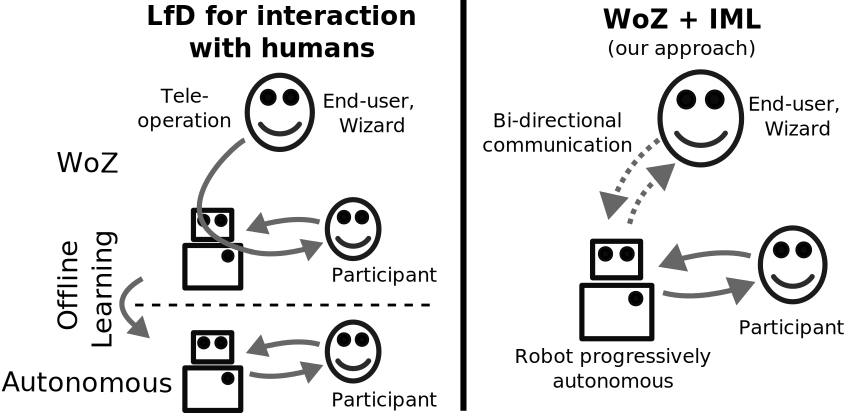
\includegraphics[width=.8\columnwidth]{figs/lfd-vs-woz2}
    \caption{Teaching a robot to interact with humans with Learning from
    Demonstration (left) is a 2 steps process with the transition between step 1
    and 2 achieved using offline learning. Our approach uses machine learning
    \emph{during} the supervision to progressively transfer the decisional
    capabilities to the robot.}

    \label{fig:lfd-vs-woz}
\end{figure}

%	\ES{running example robot tutors? - yes, but where?}
\subsection{Interactive Machine Learning}

%	\ES{Clarify advantages/drawbacks of IML and CML - currently a bit cluttered}
%IML is a term coined by Fails and Olsen in \cite{fails2003interactive}, and
%represents a move away from monolithic classical ML approach relying on a
%limited number of large learning steps. On the other hand, IML uses series of
%smaller learning steps improving the overall behaviour incrementally. 

%One of the  advantage of IML is that by relying on smaller steps, the process
%can be guided throughout the learning, speeding up the learning and leading to
%behaviour matching more precisely the desired output. Additionally, IML
%involves a human, often an end-user without technical, into the learning
%process, and this human can provide critical information to the algorithm to
%learn faster.

Interactive Machine Learning (IML), as coined by Fails and Olsen in
\cite{fails2003interactive}, is a type of learning with three characteristics:

\begin{itemize}
    \item Learn online, by interaction.
    \item Involve the end-user in the learning process.
    \item Learn by multitude of consecutive small updates of behaviours.
\end{itemize}

These three characteristics differ greatly from CML, such as Learning from the
Wizard, which uses a discrete costly monolithic learning steps ending with static
behaviours and requires numerous, and often complicated, rounds of discussions 
between domains experts and technical experts.

IML allows for simultaneous development and use of the artificial agent
\cite{amershi2014power}. By following the three principles, IML empowers the end-users 
to directly teach the agent to interact and design their own application. By removing 
the need to pass through a technical expert IML also reduces the problems of 
communication between the technical expert and the domain expert.

%Additionally, as the artificial agent is learning online, the behaviour is
%continuously updated and can be refined easily. Instead of requiring additional
%data collection, analysis rounds and long learning steps, IML allows to fine-tune a behaviour by
%simply continuing the teaching process. 

%As the robot does not require explicit learning steps once starting to learn, 
%it means that no technical expertise is required once the robot is deployed. This is radically 
%different to methods such as LfD which require technical expertise between the data 
%collection and the evaluation, and for each refinement step. 

%By involving end-users directly in the teaching process, IML removes (or
%reduces) the need of technical expertise once the robot is deployed to interact
%and learn, thus allowing end-users to obtain a learning agent and be able to
%specify its behaviour from scratch. Finally, this online teaching increases the
%transparency of the teaching process, allowing the teacher to identify more
%easily the learners' mistakes and focus their teaching on the weak points of the
%learner, with the potential of making the learning faster and more efficient.

%	have to restart a consequent part of the learning process. Similarly, when developing an	application for 
%end-users, their feedback required to improve the system can only be gathered in testing phases after each full 
%training phase and might require significant changes to the dataset or the algorithm. Finally, these approaches are 
%more sensitive to
%	differences of understanding when the developers of the application and their
%	users are from different fields \cite{amershi2014power} \ES{maybe before with advantages and drawbacks of LfD as 
%one typical example of CML}. On the other hand, IML
%	is an iterative process where the behaviour is improved at each small step, and
%	where the end-user can provide feedback on the learner's performance during all
%	these iterations. IML aims to learn faster, by continuously using inputs from
%	the end-users to correct the errors made by the algorithm as they appear thus improving the
%	knowledge gained at each learning step. Additionally, the agent learning \ES{what agent?} can also be actively 
%involved \ES{who and how?} in the process contributing to the efficiency of the approach.

One example of IML is active learning, by allowing the learner to ask questions
and query labels from an oracle for specific data points with high uncertainty,
active learning aims at improving the learning process \cite{settles2012active}.
In the context of HRI, it has been explored by having robots asking questions to
optimise a classification process \cite{chao2010transparent}. However, when
interacting in the world, the learner is not in control of which sample can be
submitted to an oracle to obtain a label. Data points are provided by the
interaction and are influenced by the learner's actions and the environment
reactions, thus limiting the potential for active learning to learn to interact. 

%Further, by learning online, IML also ease the refinement of a policy
%\SL{we should cite Maya Cakmak work on LfD integrated to joint action: when the
%	robot does not know how to do something, it 'asks' for a demonstration, and then
%	continue. Maybe this paper: "Efficient Programming of Manipulation Tasks by
%	Demonstration and Adaptation"}
%\ES{Think about difference IML, online learning, Socially Guided ML... Might be a big confusion - online=small iterations, IML=online+end-user, SGML (or two-ways IML?)=IML + feedback from robot}

%\ES{clarify what we call \woz exactly, is it just the way to supervised (IML+WoZ) or the full method?}
%\subsection{Interactive Machine Learning in the context of the Wizard of Oz paradigm} 
\subsection{Combining Interactive Machine Learning and Wizard-of-Oz} \label{sec:requirements}

%\ES{Big overlap with methods/teaching phase... - less now normally}

%\ES{Highlight that these are the requirements/opportunities for the teaching interaction}

%\ES{have more clearly defined paragraph - careful structure}

%\SL{small problem here: you've just introduced IML, it sounds great, and then
%you jump into '\woz' details (ie, our approach): I suggest in that
%section to do the 'framing' at the general IML level (including a
%quick review of what has been already done in IML to 'replace'/'complement'
%WoZ), and then, in section C, you introduce our \woz.}
%\ES{the thing is that not much as been done in that direction, I will cite munzer because it closer and other Socially Guided ML}


%\SL{By the way, from the reviewers
%perspective, there's a confusion between '\woz' and 'SPARC'. Maybe we should
%only mention SPARC as an existing technique that we reuse to realize *our* '\woz' methodology?} \ES{that's how I tried to do it, but it might be unclear}

%\ES{Maybe add more information/details on the overall method?}
In a WoZ interaction, the wizard can observe the interaction would use an interface to control the
robot. Often, these interfaces would have a large number of buttons to select
discrete actions for the robot% and potentially an open field to write utterances
%for the robot to speak out
. Combining IML and WoZ would keep the same apparatus but allow the robot to
learn from the wizard's selection of actions (considered as demonstrations) and
communicate back to the wizard (see Figure \ref{fig:lfd-vs-woz}).

The end-goal of the approach is to create an autonomous robot able to select the
actions the wizard would have taken with the same timing. This means that the
robot needs a controller with the same output as the ones available to wizard
(high level discrete actions) and the same inputs as the ones used to execute
the policy. In this context, the notion of data points for the learning
corresponds to the pair state-action for each demonstration made by the wizard.
\begin{comment}

\begin{figure}
    \centering
    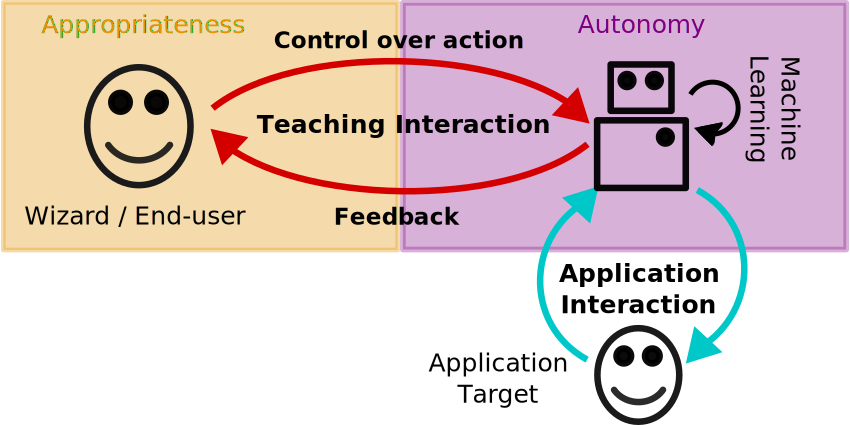
\includegraphics[width=.8\columnwidth]{figs/diagram.pdf}
    \caption{The wizard's control provides the appropriateness,
        while the machine learning on the robot and the rich bi-directional
        communication between the robot and the wizard create the autonomy. As
        proposed in \cite{sequeira2016discovering}, the wizard could also use a
        restricted-perception interface and be remotely located if required.}

    \label{fig:diag}
\end{figure}
\end{comment}

Adding IML to a classical WoZ %(as shown in Figure \ref{fig:diag}) 
creates a
complex interaction between the robot learning to interact and the wizard
teaching the robot.  In addition to the classical technical requirements of WoZ (actions
implemented for the robot, way for the teacher to perceive the interaction and
to select actions), this new interaction framework requires a perception of the
interaction state for the robot, a learning algorithm and potentially changes to 
the control interface.
%a potential overlay on
%the wizard interface to allow a bidirectional communication between the wizard
%and the robot.  

Additionally, to combine efficiently IML and WoZ, the teaching interaction needs to fit four requirements:
\begin{itemize}
    \item Interactive Online Learning: the algorithm needs to be able to be taught online to interact.
    \item Bi-directional Communication: as argued in \cite{thomaz2008teachable}, the communication channel between the teacher and the robot needs to allow for rich information (e.g. guidance and
feedback from the teacher), but the robot should also be more involved in the
teaching process and communicating back to the teacher. 
\cite{munzer2017efficient,senft2015sparc}. 
    \item Mixed Initiative: as the robot is learning as it is controlled by the teacher, 
    its knowledge on the interaction will increase, which creates the opportunity for the human 
    and the robot to fit different roles in the action selection process.
    \item Human Control: as the robot's behaviour will be imperfect while learning, the interaction
    needs to keep a key feature of WoZ -- human control. While the robot learns, the teacher needs to have 
    ways to ensure that the robot's behaviour is constantly appropriate to the current interaction.
\end{itemize}
%	These enriched demonstrations are composed of the demonstrations themselves
%	combined with a set of additional 
%information that can be used to improve the learning, making it faster and more
%precise (in a fashion similar to \cite{basu2018learning} \ES{discuss how}, but
%where the feature would be provided directly with the demonstration).
%\ES{repetition}
\begin{comment}

As argued in \cite{thomaz2008teachable}, the communication channel between the
teacher and the robot needs to allow for rich information (e.g. guidance and
feedback from the teacher), but the robot should also be more involved in the
teaching process and communicating back to the teacher. Having the robot provide
feedback to the wizard can increase the transparency of the teaching process 
%\ES{clarify before that the system is not passive with IML}
, improving the wizard's behaviour and in some context contribute to providing
autonomy by proposing actions to support the wizard
\cite{munzer2017efficient,senft2015sparc}. 

%Furthermore, this feedback could be used to support the wizard in the control,
%potentially reducing their workload.  \ES{would that be clearer?} \SL{not super
%clear for someone that does not know yet what SPARC is: whatis different from
%normal WoZ? why? how? what do you mean by 'enrich selections'for instance?}. 

%\subsection{Requirements on the Teaching Interaction} 

%During the teaching phase, the wizard interactively teaches the robot a policy
%suitable for the current application.  Figure~\ref{fig:diag} presents the
%combination WoZ and IML: the robot interacts with a target, is controlled by the
%wizard (providing both appropriateness and adaptivity) through a dedicated interface and
%the robot learns from this control, providing the wizard with
%feedback on the learning process (providing the autonomy)\SL{it sounds like 'the
%feedback provides autonomy', which is probably not what you mean} \ES{actually, it can, especially in the case of SPARC}. This communication
%between the wizard and the robot might follow the concept of \emph{socially guided
%machine learning} \cite{thomaz2008teachable}, whereas, unlike classical LfD, the
%robot provides the teacher with additional information on its intentions,
%confidence or learning state which increases the transparency and the efficiency
%of the teaching process.



The state perception needs to capture all the features required to select
actions efficiently. The learning algorithm needs to be able to receive
demonstrations and learn quickly as interacting in the real world implies a slow
and costly accumulation of data. Furthermore, it needs to provide feedback to
the wizard to improve transparency beyond the simple observation of the robot's
behaviour. Similarly, the interface needs to allow for this bi-directional rich
communication. Finally, as the actions required for \woz are the same as the
ones used by the wizard in a classical WoZ, no modification is required on the
action side.

%\ES{better?}
%\SL{again, not clear why
%the wizard needs the algo feedback directly: one would expect that the algo %feedback is
%actually the resulting robot behaviour... need to explain that}. 
%	Furthermore, as the
%	robot interacts at a human timescale and in the real world, collecting data points can be slow and costly process. 
%Consequently, to be useful, the algorithm needs to make a maximum use of the teacher's presence and be able learn from 
%a highly limited number of data points.
% \ES{good comment Sév, better?}
%\SL{sentence
%implies 'online learning $\Rightarrow$ highly limited number of data point' which is not
%quite true. The problem is rather that because we interact with the actual end
%user, we can not easily repeat the same interactions, and because the all approach
%is only valuable if the robot learns relatively quickly, we do not have a lot of
%data points to learn from}.

This combination of WoZ and IML could start in the same way as classical WoZ
(and methods based on LfD for teaching interaction with humans
\cite{knox2014learning,	sequeira2016discovering}), but quickly, as the robot
receives demonstrations and feedback and learn, it could increase its autonomy.
This relation between human control and robot autonomy can be made using
mixed-initiative control, and as the robot improves its policy, it has the
potential to reduce the workload on the wizard. The goal of this combination is
to maintain a high appropriateness in the application interaction while
progressively increasing the robot's autonomy.  Figure~\ref{fig:concept}
presents an ideal comparison between WoZ, LfD and WoZ combined with IML in term
of autonomy and appropriateness. It should be noted that this ideal comparison
only aims to provide readers with an intuition of the key aspects of \woz and is
not supported by data from studies in the real world.


%\ES{why presenting ideal if it will never happen? - see comment from reviewer}
%what is the use / worth of the comparison of ideal situation if this is never
%going to look like this? For example, human wizards are not perfect (so
%adaptively and appropriateness fluctuates). The assumption that autonomy will
%be flawless doesn’t make sense. Where are you getting the idea from that the
%transfer of autonomy will be an exponential process? How will appropriateness
%and adaptive be operationalized? These are all big questions that are left
%unanswered / overlooked by presenting this model. The reviewer believes this
%model does more damage to the story than it does good.



%\SL{might become hard to read, but would be really useful to plot the
%'adaptability' as well, as it would show the LfD is not adaptable. Maybe
%'autonomy and adaptability' together?}.  \ES{replace performance by
%`appropriateness and adaptivity', better?+ added the concept of refinement step
%- might be too much??} The goal of this combination is to maintain a high
%appropriateness in the application interaction while progressively increasing
%the robot's autonomy, reducing the workload on the wizard and eventually
%leading to a fully autonomous behaviour if required.  Compared to LfD
%approaches such as the one proposed by Sequeira et
%al.~\cite{sequeira2016discovering}, this method has three main advantages.
%First there is no engineering step between demonstrations collection and the
%autonomous phase (improving usability), second, by involving both the wizard
%and the artificial agent in the learning process, the learning is faster and
%transparent, and third, even after the teaching phase, the wizard can easily
%step back in the teaching loop in further interactions to refine the robot's
%behaviour. \ES{not in line with model presented before}
%	

\begin{figure}
    \centering
    \includegraphics[width=1\columnwidth]{figs/concept.pdf}
    \caption{Idealised comparison of appropriateness and autonomy over
        time for three methods: WoZ, LfD and WoZ+IML. With LfD, after the learning step, the behaviour is static 
        and with limited appropriateness, multiple refinements steps are required to evaluate and improve the 
        appropriateness.
        %    \SL{Adaptivity should be much
        %    lower on the LfD graph, and refinement steps should increase the human
        %    workload, no?}
    }
    \label{fig:concept}
\end{figure}

\end{comment}
%\ES{I'm still unconvinced that it should focus strongly on SPARC and one
%implementation already... Because this is supposed to be more generalisable,
%even SPARC is only one way to do it - I feel that commiting to SPARC at that
%point potentially reduce the usability of the paper, as it would be relevant
%only for the people using sparc already - for example the paper from sequeira
%et al. does not have any equation or algorithm, it is a general method with one
%example of application}

%	\subsection{Mixed Initiative Control} \label{sec:sparc}
%	
%	\ES{Define Supervised autonomy first as the desire on our mixed initiative control, and then relate to sparc}
%	
%	\ES{probably focus more on mixed initiative control - refer to Sheridan's scale of autonomy? not to the method yet 
%- this talks about WoZ+IML!}
%	
%	\ES{Maybe mention first the idea of progressive autonomy, and then how you could achieve it}
%	
%	%\ES{more distance sparc and now - maybe only supervised autonomy!}
%	
%	One of the key consideration when combining IML and WoZ is to keep the teacher in control
%	of the robot behaviour as this is the only way to ensure the appropriateness of actions.
%	However, as the robot improves its autonomy over time, and we would like this to reduce 
%	the teacher's workload, the robot's behaviour should follow a mixed-initiative control
%	where both the robot and the teacher can impact the executed behaviour. 
%
%\ES{supervised autonomy and level of autonomy}
%	The Supervised Progressively
%	Autonomous Robot Competencies (SPARC) framework~\cite{senft2015sparc} is an approach for IML to put the end-user in 
%the teaching loop, using the concept of \emph{supervised autonomy}.
%	
%	%Instead of segmenting a demonstration or coding part and a fully autonomous
%	%part, we propose the \woz methods, a way to use IML to smoothly move away
%	%from WoZ to full autonomy. This method aims to allow researchers to actively
%	%teach robots autonomous behaviour without requiring technical expertise. That
%	%way, teachable setups could provide a base of experiment used by numerous
%	%researchers to explore different sides of the interaction without requiring any
%	%technical expertise to design an autonomous behaviour. Additionally, as this
%	%behaviour derives from online teaching, they might be more transparent, further
%	%improving the user experience \cite{amershi2014power}.
%	
%	\begin{figure*}
%		\centering
%		\includegraphics[width=\textwidth]{figs/sparc_overview.pdf}
%		\caption{Overview of the action selection flow for SPARC. Mixed initiative
%			is achieved by allowing the robot to propose actions to the wizard (that the
%			wizard can accept or discard) while letting the wizard select actions
%			him/herself as well. The ``Action should be selected'' box corresponds to the action selection process 
%(including the algorithm) which might decide to propose an action to the wizard or not.
%			%\SL{what is the first box 'action should be selected?'}
%			%\ES{better?}
%		}
%		
%		\label{fig:overview}
%	\end{figure*}
%	
%	%\subsubsection{Overview}
%	%SPARC is an approach designed to allow end-users to teach robots to interact in
%	%sensitive environments such as HRI.
%	%The setup used by SPARC is similar to that
%	%of WoZ, except that the robot learns from the wizarding and can propose actions
%	%to the wizard. 
%	
%	The main feature of SPARC makes it fit the requirements \ES{are those explicit?} presented in the previous
%	section. First, the wizard is continuously in control of the robot behaviour:
%	the wizard can select actions for the robot to execute (in a fashion similar to
%	WoZ), but the robot can also propose actions to the wizard, which will be
%	executed after a short delay if not cancelled. Thus, each action executed by the
%	robot would have been either selected or passively approved by a human. This
%	automatic execution also allows the workload on the wizard to decrease as the
%	robot learns. Figure \ref{fig:overview} presents an overview
%	of the mixed initiative control provided by SPARC. SPARC can be used with augmented demonstrations and combined 
%with a
%	wide range of algorithms and as such the action selection step and the update
%	of policy can vary widely.
%	
%	The conceptual and algorithmic framework introduced by~\cite{senft2015sparc} forms the framework for the teaching 
%interaction in our \woz methodology, that we present hereafter.

\section{\woz Methodology} \label{sec:method} 

\begin{figure*}
    \centering
    \includegraphics[width=\textwidth]{figs/timeline.pdf}
    \caption{Timeline of WoZ, LfD (WoZ to create a dataset and the ML to learn a behaviour) and WoZ++. 
    }
    \label{fig:timeline}
\end{figure*}

%	\ES{SPARC is one possible interaction framework for WoZ++}

%	\ES{Add timeline for IML vs CML with domain expert vs technical expert? or in discussion or nowhere?}

%	\ES{Highlight that the human is actively teaching!!!}
%	
%	\ES{Should we compare already to LfD?}

%	\ES{give high level procedure and goal in intro??}

This section presents \woz, a new method to allow end-users (in our case HRI
researchers or members from the general public) to create fully autonomous robot
behaviours. \woz is composed of two main phases: the \emph{implementation phase} and the \emph{teaching phase}. Figure \ref{fig:timeline} presents the timeline of \woz as well as classical WoZ and CML, using Woz to collect data and then applying machine learning on these data (e.g. Learning from the Wizard \cite{knox2016learning}).

%We start to describe the teaching phase as this is the key part of
%\woz and it guides the 
%elements that will need to be implemented in the implementation phase.
%Throughout this section, we will take as a case study the one
%proposed in \cite{senft2018robots}, to which we applied \woz to reach an
%efficient autonomous robot behaviour.

%Throughout this section, we will follow the example of a team of researchers
%exploring the impact of the sociality of a robot's behaviour on children
%behaviour in the context of freeplay-sandbox as proposed in
%\cite{lemaignan2017free} and more specifically, the educational task presented
%in . 
%The study followed the Sandtray paradigm \cite{baxter2012touchscreen}, a child
%and a robot are sitting on opposite sides of a touchscreen where an educational
%application is displayed. The robot can guide and support the child in the
%activity by analysing the inputs on the screen and providing game related
%information. In that study, 10 animals and 11 plants were displayed on the
%screen with some energy and the animals had to be fed to be kept alive. The
%child needed to move animals toward other animals or some plant to feed them,
%and consequently could learn what animals eat. The robot could provide hints and
%social feedback to the child to improve their behaviour in the game. It should
%be noted that this paper does not aim to describe this study in details, but
%rather to use it as an example of how \woz could be applied and to demonstrate
%that \woz can be efficient in the real world. More details and results can be
%found in \cite{senft2018teaching} and the sources and data for this paper are
%available online
%\footnote{\url{https://emmanuel-senft.github.io/experiment-woz-plus-plus.html}}. 

\subsection{Implementation phase}

The goal of \woz is to allow non-technical users to teach a robot an interactive
behaviour by combining IML and WoZ. The core of this method is the teaching
phase, the phase in which the wizard actively teaches the robots. However, to be
able to teach the robots, all the tools required for the interaction first need to be implemented. This implementation phase is divided into three steps: defining the
world representation, selecting the algorithm, and selecting the interaction
framework and the interface between the robot and the teacher. These three
first steps do require technical expertise to implement the associated software
elements, and have to be completed before the teaching phase starts. However,
once the teaching starts, no further technical expertise is required to reach
autonomous behaviour if desired.

%The researcher are experts in cognition and social behaviours but have limited
%knowledge in computing, and they aim to explore how the robot's social
%behaviours impact the child in a game or a test. \ES{mention that it's fairly
%common?}

%\subsection{Overview}
%\ES{intuition}

\subsubsection{Definition of World Representation}

The first step in \woz is collecting information about the type of behaviour
required by the robot to interact efficiently in the application (the analyse of the application domain in Figure \ref{fig:timeline}). This
collection can be from discussions with domain experts: such as therapists or
teachers in the case of education, or by staging mock up studies involving
human-human interactions and collecting data from the field, as proposed in
\cite{sequeira2016discovering}.

Then, the inputs (processed sensory inputs and interaction features) and outputs
(actions) available to the controller need to be selected and implemented. This
step is common for \woz and LfD as the learning algorithm will have to assign an
action for each possible state for both cases.  On the other, WoZ only requires
the definition and implementation of the actions.

\begin{comment}
For example, Table \ref{tab:state_space} presents the state space (type of
inputs available to the algorithm) used in the case study, and the outputs of
the algorithm, the game actions, are presented in Table \ref{tab:actions_space}.
In total, this case study corresponded to an optimisation task assigning one or
none of 655 actions to each possible point in a 210 dimensional space (with real
values ranging from 0 to 1).

\begin{table}[ht]
    \centering
    %	\ra{1.4}
    \caption{Definition of each category of the state space. Items correspond to
    all the elements of the game: the 10 animals and the 11 plants.}

    \label{tab:state_space}
    \begin{tabularx}{\columnwidth}{@{}L{.65}L{1.05}L{.15}L{2.15}@{}}\toprule
        Group & Name & \# & Description \\
        \midrule
        Game State & Distance Between Items & 155 & Normalised distance between the animals and each other animal 
        and the plants.\\
        & Items' Energy & 21 & Energy of the 21 items.\\
        & Progress in the Game & 1 & 0.25 for first game to 1 for the last game.\\ 
        Temporality & Robot Touches & 10 & Time since the robot touched each animal.\\ %decay
        & Child Touches & 10 & Time since the child touched each animal.\\ %accumulation
        & Task-Specific Events & 3 & Time since last eating event, failed interaction and death of any animal.\\ 
        %decay
        & Robot Actions & 5 & Time since last robot action of each type.\\ %decay
        & Generic Last Actions & 2 & Time since last child touch and last robot action of any type.\\ 
        %decay\accumulation
        Child state & Focus & 3 & Time since last child's gaze facing the robot, the screen and outside.\\ 
        %accumulation
        \bottomrule
    \end{tabularx}
\end{table}

\begin{table}[ht]
    \centering
    %	\ra{1.2}
    \caption{Definition of each category of the action space. Each action is
        associated to a verbal utterance selected among 5 possible ones.}
    \label{tab:actions_space}
    \begin{tabularx}{\columnwidth}{@{}lllX@{}}\toprule
        Type & Name & \# & Description \\
        \midrule
        Game Actions& Move close & 210 &  Action moving any animal close to any item.\\
        & Move to & 210 & Action moving any animal to any item.\\
        & Move away & 210 & Action moving any animal away from any item.\\
        & Remind rules & 1 & Verbal utterance.\\
        Social Feedback & Congratulation & 1 & Verbal utterance.\\
        & Encouragement & 1 & Verbal utterance.\\
        Hint & Attention & 21 & Drawing the child's attention to any item.\\
        Meta-level & Wait & 1 & Doing nothing.\\
        \bottomrule
    \end{tabularx}
\end{table}
\end{comment}

\subsubsection{Teaching Framework}	

\label{sec:framework}
The second element to define before the teaching phase is the interaction
framework between the robot and the teacher. By combining WoZ and IML, the
teacher should be able to select actions for the robot to execute, but the robot
is also expected to increase its autonomy, this results in a mixed-initiative
scenario where both the robot and the teacher should be able to influence the
executed behaviour.

However, one important consideration with \woz is that we would like the robot's
appropriateness to be at human-level during each step of the interaction,
especially during the teaching phase. Consequently, the human should
continuously remain in control of the robot's behaviour.

This results into three requirements on the teaching framework:
\begin{itemize}
    \item Keep the teacher in control of the robot
    \item Allow mixed-initiative between the teacher and the robot
    \item Allow rich bi-directional communication between the teacher and the robot
\end{itemize}

Additionally, and as shown in Figure \ref{fig:timeline}, the interface between the 
teacher and the robot corresponding to the interaction needs to be implemented too.

\begin{comment}
In this study, we used the \emph{supervised autonomy} to achieve this.
Supervised autonomy is a mix between tele-operation (the wizard can select
actions for the robot) and the level 6 on Sheridan's scale of autonomy
\cite{sheridan1978human}: ``Computer allows the human limited time to veto
before automatic execution''. This allows both the teacher and robot to select
actions, and give the teacher the opportunity to prevent the robot from
executing undesired actions.  With the addition of the learning component of the
robot, this correspond to Supervised Progressively Autonomous Robots
Competencies (SPARC)\cite{senft2015sparc}, an interaction framework designed
especially to allow teachers to share control with a learning agent (see Figure
\ref{fig:overview}).

\begin{figure*}
    \centering
    \includegraphics[width=\textwidth]{figs/sparc_overview.pdf}
    \caption{Overview of the action selection flow for SPARC. Mixed initiative
        is achieved by allowing the robot to propose actions to the wizard (that the
        wizard can accept or discard) while letting the wizard select actions
        him/herself as well. The ``Action should be selected'' box corresponds to the action selection process 
        (including the algorithm) which might decide to propose an action to the wizard or not.
        %\SL{what is the first box 'action should be selected?'}
        %\ES{better?}
    }
    \label{fig:overview}
\end{figure*}

It should be noted that other approaches such as the ones from
\cite{chernova2009interactive,munzer2017efficient,thomaz2008teachable} could
also be used as interaction framework instead of SPARC, but we selected SPARC as
it is specially designed to keep the wizard in control of the robot's behaviour,
while leaving space for the robot to learn and should lead to an efficient
learning compared to other methods \cite{senft2017supervised}. Regardless of the
teaching framework selected, and similarly to other methods based on WoZ, an
interface between the wizard and the robot needs to be implemented and fit the
specificities of the teaching framework.
\end{comment}

\subsubsection{Algorithm Selection}\label{sec:algo}

%\ES{could make it smoother and clearer}
The last element which needs to be selected and implemented is the learning 
algorithm.
Not all algorithms could be used with \woz. The main specificity is that the
algorithm needs to be compatible with IML, so learning steps needs to be short 
and the algorithm needs to be able to generalise quickly from a limited number 
of datapoints. Many algorithms can learn online: for example 
instance based algorithms (e.g. Nearest-Neighbours \cite{cover1967nearest}) or 
algorithm in the Reinforcement Learning (RL) family \cite{sutton1998reinforcement}.
However, these algorithm should make a fuller use of the interactive teaching 
offered by the method, for example by using additional meta-information from the 
teacher (e.g. additional feature to quicken the learning or modifications of learning meta-parameters) and provide the teacher with information about the status of the learner
(e.g. intended behaviour, confidence in action, perception of the
world...).
%However, some features might be required to be able to 
%generalise faster than classical versions as acquiring datapoints from the real 
%world can be a slow process. Nevertheless, the active presence of the teacher 
%provide the algorithm with the opportunity to obtain meta-information about 
%the learning environment not available in other types of interaction. \ES{probably more details here}
%Additionally, as explained in [ref to bidirectional], the algorithm needs to be
%able to provide the teacher with additional information about the state of the
%learner according to the teaching framework (such as expected behaviour, confidence in action, perception of the
%world...).

This results into four requirements for the learning algorithm:
\begin{itemize}
    \item Learn online
    \item Generalise quickly 
    \item Able to use meta-information from  the teacher
    \item Feed back information to the teacher
\end{itemize}

\begin{comment}
With \woz, the learning algorithm needs to be applicable to learn online, from
the first data point, and also be able to learn quickly and efficiently to reach
an appropriate policy in a human timescale. 

Instance-based algorithms, such as Nearest-Neighbours \cite{cover1967nearest},
are specially adapted to online learning from a limited number of data points.
However, in the classical version, the use of each instance accumulated is basic
and might contain unnecessary information, limiting the learning speed. For such
reasons, in the study, we used an algorithm designed to use augmented
demonstrations (with features used to keep only the relevant information) and
the wizard's feedback on propositions to allow for fast learning of policies in
complex, multidimensional states. 

The algorithm used in the study is presented in Algorithm \ref{algo:algo} and is
inspired from \cite{senft2017toward}). It uses as instances tuples ($a,s',r$)
composed of the action evaluated by the wizard ($a$), a substate ($s'$) and a
reward related to the selection of this action in that substate. This algorithm
has three key differences compared to classical Nearest Neighbours: first the
instances are defined on substates, which are states vectors defined only on a
limited number of dimensions of the full state space, with the other dimensions
left as wildcards. This allows to consider only the parts of the state that are
relevant to the actions when computing the distance between the current state
and each instance in memory. The dimensions retained for each substate are
inferred from features provided by the wizard with the demonstration. Thus, the
algorithm can learn rich behaviours quickly, even in large state spaces,
increasing the range of behaviours allowed with a single world representation
and a single algorithm. The second addition to classical Nearest-Neighbours is
the concept of rewards associated to a state-action pair (which is inspired from
Reinforcement Learning \cite{sutton1998reinforcement}). This allows to select
the actions already demonstrated by the wizard, while avoiding the ones the
wizard deemed not appropriate.  Finally, in most of the states, no action should
be executed, consequently, actions are only selected when their expected reward
(the multiplication of the reward value by the distance to the current state) is
higher than a threshold. This threshold is updated when the wizard evaluates an
action. 

\ES{Should I add more details on the algo: potential and limits? more comparison with NN, 
robustness? - there were many comments from the reviewers on that, but it's quite out of topic 
and could add confusion and divert the reader from the important points of the paper.}
%\ES{expend discussion on algo? what it can do or not do? - here on in discussion?}
%\ES{clarify why algo vs NN and what if inconsistency in demo but maintain limits of PSNN}
%\ES{it can generalise quickly, but when enough data points, each has a limited impact + teacher in the loop}
%\ES{maybe clarify what the algorithm need and then why this one would satisfy this}
\begin{algorithm}
    \DontPrintSemicolon
    \SetKwInOut{Input}{inputs}\SetKwInOut{Output}{output}
    \Input{
        $s$: current state\\
        $C$: collection of instances $c = (a,s',r)$\\
        $A$: ensemble of actions present in $C$}
    \Output{selected action $\pi(s)$}
    \ForEach{$a \in A$}{
        \ForEach{$p=(s',r) \in C_{a}$}{
            compute similarity $\Delta$ between $s$ and $s'$:
            $\Delta(p)=1-\frac{\sum_{i \in N' }(s'(i)-s(i))^{2}}{n'}$
        }
        find closest pair $\hat{p}$:\\
        $\hat{p} = arg\, max_{p} \Delta(p)$\\
        compute expected reward $\hat{r}(a)$ for taking $a$ in $s$:\\
        $\hat{r}(a) = \Delta (\hat{p}) \cdot r(\hat{p})$\\
        with $r(p)$ the reward $r$ of the pair $p = (s',r)$ 
    }
    Select the action with the maximum expected reward:
    $\pi(s) = arg\, max_{a} \hat{r}(a)$

    \If{$\hat{r}(\pi(s)) >$ threshold}{
        Propose $\pi(s)$ to the wizard
    }	
    \caption{Algorithm for selecting an action based on the previous instances
        tuples (action, substate, reward) and the current state. Substates (s') are
        defined on a subset of the state space, with N' the ensemble of the n'
        indexes of the retained dimensions of s' \cite{senft2017toward}.}

    \label{algo:algo}
\end{algorithm}
\end{comment}

\subsection{Teaching Phase}

%	\ES{Discuss teaching paradigm}

%	\ES{introduce before that the human is teaching from WoZ ><}
The main step with \woz is the teaching phase, the one where
the robot is taught an interactive behaviour. Based on Socially Guided Machine
Leaning \cite{thomaz2008teachable} and IML \cite{amershi2014power}, \woz applies
interactive online learning to the creation of social interactive policies for
robots. Figure \ref{fig:setup} presents the setup used in the teaching phase in
the two case studies: a wizard controls and teaches the robot through a graphical user
interface running on an external laptop or a tablet, while the robot is
interacting with another human. As mentioned in Section \ref{sec:requirements}, to combine WoZ and IML, \woz relies on four characteristics: interactive online learning, bi-directional communication, mixed-initiative and human control.


%However, unlike classical WoZ or LfD, the robot has a way to communicate
%feedback to the wizard and learns online from the demonstrations and inputs
%from the wizard. This enriched two ways communication aims at giving more tools
%to the wizard in the teaching and informing them about the learning state of
%the robot (thus increasing transparency of the teaching process). Additionally,
%this feedback channel from the robot to the wizard can be used to convey
%robot's intentions and alleviate the wizard's workload, for example by
%proposing actions to the wizard as used with SPARC.

%In the case study proposed, the interaction between the robot and the wizard
%was done using SPARC (Supervised Progressively Autonomous Robots Competencies)
%\cite{senft2015sparc}. The wizard had access to an interface representing the
%state of the game played by the child and the robot. Using this interface, the
%wizard could select actions for the robot to execute and select the features of
%the environment relevant to the action selection. Additionally, the robot could
%propose actions through the interface, which would be executed automatically
%after a short delay, enforced by the wizard or simply cancelled. Using the
%feedback on propositions, the selection of actions and the associated features,
%the learning algorithm could learn an appropriate behaviour. 



%\ES{Kind of repetition...}
\subsubsection{Interactive Online Learning}

The first key consideration when applying \woz and the main focus of this paper
is the interactive online learning: the wizard needs to be able to teach the
robot online an efficient policy. The teaching interaction needs to happen in the real world,
directly in the domain the robot is expected to interact in. The learning 
needs to start from the first demonstration and use any type of information it can 
get from the teacher or the environment. And both the teacher and the robot need
to be actively involved in the teaching/learning process and communicate between each other.

%The communication needs to be both ways
%between the wizard and the robot to make the learning more efficient and
%increase the transparency of the teaching interaction (between the wizard and
%the robot).  This communication depends of the interaction framework selected.

%and could implement a mixed initiative control, whereas both the
%wizard and the robot are involved in the action selection process, and both
%provide additional information to the other party. 
%Additionally, the wizard could have access to a `Restricted Perception'
%interface representing the state of the world as seen by the algorithm (as
%proposed and advocated in \cite{sequeira2016discovering}). The robot should also
%communicate information on its learning status and its intentions, and could
%propose actions for the wizard to execute and use its confidence to impact the
%way the action is proposed to the wizard \cite{chernova2009interactive}.

%In the study, the interaction was following SPARC and the algorithm was the one	presented in Algorithm \ref{algo:algo}. \ES{clarify difference with sparc}
%In the study, we used SPARC to handle the mixed initiative and for methodological 
%convenience, we did not use a restricted perception.
%The teacher was in the same room as the interaction and observed the child 
%and the robot interacting.
\subsubsection{Bi-directional communication}

As explained previously, to profit fully from the teacher's presence, the 
communication between the teacher and the robot needs to go both ways.
First, the robot needs to inform the teacher about its status (vision of the world,
learning state, intentions, confidence \ldots). But the teacher needs also to communicate 
rich information to the robot (demonstrations, meta-information, feedback on intentions  \ldots
This rich bi-directional communication aims to make the teacher process faster and more
efficient, but also more transparent, keeping the teacher aware of the state of the learner.

%\ES{augmentation of demonstration and feedback from the robot, meta-parameters..}

%\ES{more details here? and not before}	
%Using the interface, the wizard can select actions for the robot to execute
%(similarly to WoZ), as a form of demonstration. However, one important point is
%that these demonstrations should not be simply the action selected by the
%wizard, but should be joined by additional information to speed up the learning.
%In the study, we decided to add to each demonstration a set of features explaining
%their choice, but other methods could be used. %For example, in \cite{basu2018learning}, 
%authors propose to allow the teacher to augment a comparison between two trajectories with
%a feature explaining their choices, alternatively, \cite{mueller2018robust} propose to add
%constraints to demonstrations. 
%These meta-information aim to make the teaching process faster and more efficient.
%    The wizard could highlight
%	features of the environment when selecting an action (such as animals or plants)
%	and the learning algorithm would infer the dimensions of the state space related to
%	these features, discarding the irrelevant information to achieve faster learning.

\subsubsection{Mixed Initiative}

Using \woz, the wizard-robot team can vary its position on the autonomy
scale: from fully autonomous robot to full tele-operation.
% (such as WoZ) \ES{reviewer does not like to say that woz is full teleoperation}. 
As such, the wizard can be in control of the robot's level of autonomy, starting
with a low autonomy in the early stage of the learning to a total one when the
robot has received enough demonstrations to express an efficient policy. By
increasing the robot's autonomy, the wizard can also alleviate their workload,
making the wizarding process more lightweight and comfortable.

%This way of interacting is aimed to allow for a quick learning, leveraging
%human's skills at teaching agents, and potentially requiring a reducing
%workload from the wizard as the robot learns and take over part of the action
%selection. 

\subsubsection{Human Control}

Finally, the wizard needs to be in control of the robot's behaviour. Regardless
of the interaction framework selected, as the robot learns to interact, its
policy is imperfect and would lead to inappropriate behaviour.  Thus the human
needs to have oversight on the robot's behaviour to ensure that it constantly
achieves a human-level appropriateness. This consideration is especially
critical as the robot is being to taught to interact with humans in the real
world, where its actions have real impacts and might cause harm or distress to
its partner. 

%	This
%	is one the main consideration of SPARC: by forcing each action to be approved
%	(actively or passively) by the wizard, the robot's behaviour during the teaching
%	phase can be assumed to be on a similar level with one expressed using WoZ. 
%	\ES{reviewer: I disagree, passively accepting a selected action is not as good as actively selecting an action. 
%Humans will lose attention if they feel the system is taking care of stuff for them. See the self-driving car 
%discussion.”} 

%\ES{supervised autonomy and level of autonomy}
%The Supervised Progressively
%Autonomous Robot Competencies (SPARC) framework~\cite{senft2015sparc} is an approach for IML to put the end-user in 
%the 
%teaching loop, using the concept of \emph{supervised autonomy}.
%
%	The main feature of SPARC makes it fit the requirements \ES{are those explicit?} presented in the previous
%	section. First, the wizard is continuously in control of the robot behaviour:
%	the wizard can select actions for the robot to execute (in a fashion similar to
%	WoZ), but the robot can also propose actions to the wizard, which will be
%	executed after a short delay if not cancelled. Thus, each action executed by the
%	robot would have been either selected or passively approved by a human. This
%	automatic execution also allows the workload on the wizard to decrease as the
%	robot learns. Figure \ref{fig:overview} presents an overview
%	of the mixed initiative control provided by SPARC. SPARC can be used with augmented demonstrations and combined 
%	with a
%	wide range of algorithms and as such the action selection step and the update
%	of policy can vary widely.
%	
%	The conceptual and algorithmic framework introduced by~\cite{senft2015sparc} forms the framework for the teaching 
%	interaction in our \woz methodology, that we present hereafter.

%Instead of segmenting a demonstration or coding part and a fully autonomous
%part, we propose the \woz methods, a way to use IML to smoothly move away
%from WoZ to full autonomy. This method aims to allow researchers to actively
%teach robots autonomous behaviour without requiring technical expertise. That
%way, teachable setups could provide a base of experiment used by numerous
%researchers to explore different sides of the interaction without requiring any
%technical expertise to design an autonomous behaviour. Additionally, as this
%behaviour derives from online teaching, they might be more transparent, further
%improving the user experience \cite{amershi2014power}.

\subsection{Beyond Teaching}
%	\ES{clarify role of the study + requirement to stop + not yet talk about refinement}

\subsubsection{Autonomous Interaction}

\woz can be used to create a fully autonomous behaviour if desired.  Once the
robot is deemed to have a sufficiently correct behaviour, the teaching phase can stop.
In that case, the robot can either be left to interact autonomously or be
kept under supervision depending on the context of interaction.  
%If further
%refinement steps	are required, the wizard can simply step back in control and
%continue the teaching process. 
As the robot learns online to interact, the autonomous deployment is
straightforward: the robot can directly use the output of its algorithm.
Additionally, the learning component can either disabled, or replaced by an
autonomous one such as Reinforcement Learning \cite{sutton1998reinforcement}. 

\begin{comment}

In the case study, we used \woz to teach the robot to support children in the
educational activity. After the teaching phase which consisted of interaction
with 25 children, we evaluated the robot's taught policy in interactions with 25
other children to test if the teaching was successful. To create the autonomous
behaviour, we used a module automatically accepting the algorithm suggestions
after a short delay. 

\ES{cut down details}
Figures \ref{fig:supervised} and \ref{fig:autonomous} show the different
policies (number of actions per category and per child) applied by the robot
under human supervision or when interacting autonomously. Despite some
differences (e.g. the autonomous robot doing more encouragement while the wizard
used more congratulations), the two policies present similarities (more social
actions than other actions, limited use of move away and no use of move to). The
difference of policy is to be expected with the diversity of the children and
the risk of bias toward certain instances with instances-based algorithms,
especially as it was observed in the study that the teacher did not have a
strict a clearly defined policy. For example, she used the actions encouragement
and congratulation in similar situations, which presented challenges for the
algorithm to match precisely the teacher's behaviour.

%In that case, the main
%difference was between two actions with similar impacts: encouragements (e.g. ``Keep going'') and
%congratulation (e.g. ``Well done''). As the game was high pace with repetitions of the same event multiple times
%through a session and the teacher did not have a strict and simple policy, 
\ES{Is this enough? or should I do more?}
%\ES{clarify that as fast pace, harder to capture a clear cut/sometime encourages used after eating event (-check-)}

%\ES{Is this the best place for results, or should they be somewhere else? - and how to balance with discussion - and is it enough to support that the method is effective}
\begin{figure*}[ht]
    \centering
    \begin{subfigure}[b]{1\columnwidth}
        \centering\includegraphics[width=1\columnwidth]{figs/supervised_actions.pdf}
        \captionsetup{width=.95\linewidth}
        \caption{ Number of actions executed by the robot per type and per child, when the wizard taught the robot.\label{fig:supervised}}
    \end{subfigure}%
    \hfill
    \begin{subfigure}[b]{1\columnwidth}
        \centering\includegraphics[width=1\columnwidth]{figs/autonomous_actions.pdf}
        \captionsetup{width=.95\linewidth}
        \caption{Number of actions executed by the robot per type and per child, when the robot was autonomous (the children in that condition were different than the ones when the robot was teaching).\label{fig:autonomous}}
    \end{subfigure}
    %\caption{\subref{fig:fig1} shows Figure~1 and~\subref{fig:fig2} shows Figure~2.}
    \caption{Number of actions of each types executed by the robot per child (top row supervised robot, bottom row autonomous robot).}
    \label{fig:policy}
\end{figure*}

Additionally, Figure \ref{fig:timing} shows the time between each action
executed by the robot and the last eating event. This graph demonstrates that
the learning algorithm captured time dependencies between events and actions.
For example, it can be observed that the teacher only used the `Congratulation'
action shortly after this type event, while the `Move close' action was also
used much later after this type of event.  As shown by the similarity of
distribution between the supervised robot and the autonomous one, the autonomous
robot learned this pattern and was able to replicate it in its policy.

\begin{figure}
    \centering
    \includegraphics[width=1\columnwidth]{figs/timing_actions_animal_eat.pdf}
    \caption{Timing between each action and the last eating event (due to their
    low or null number of execution, the actions `Move to' and `Move away' were
    not analysed).}

    \label{fig:timing}
\end{figure}

%\begin{figure} \centering
%	\includegraphics[width=1\columnwidth]{figs/compa_time.pdf} 
%	\caption{Difference between the congratulation action and the last eating interaction done by the child for the robot being taught or interaction autonomously.} 
%	\label{fig:compa}
%\end{figure}

%The game consisted on 4 rounds of slightly under 2 minutes per participants
%(children of 8 to 10 years old). The teaching phase was run with 25 children
%and used a wizard with limited technical knowledge. The testing phase contained
%25  children and a third group of 25 children interacted with a passive robot
%to serve as a control condition. Figure \ref{fig:setup} presents a picture of
%the system being used to teach the robot to interact with a child.  not simply
%applying offline learning on tasks but using human skill to \textbf{teach}
%robot

%richer 2 ways communication - online learning - relation to socially guided
%machine learning \cite{thomaz2008teachable}

%\ES{big emphasis on online learning}
\end{comment}

\subsubsection{Supervised Autonomy}

Alternatively, instead of being fully autonomous, the wizard could constantly
keep an oversight role whereby they ensure the robot is acting correctly while
not having to select each action manually. This could be required if removing
totally the human from the action selection loop raises risks or ethical
concerns, such as when using robots in therapies. In that case, the wizard could
maintain the teaching interaction, staying in control of the robots's behaviour,
but as the robot's behaviour should already be correct, their workload should be
reduced.

Additionally, in some cases the robot might need to express a different policy
than the one it has been taught: for instance if the robot learned to interact
with typical children but the current child has special needs. As the
interaction between the robot and the wizard already allows the wizard to be in
control of the robot's action, the wizard could  step back in the
action selection loop, ensuring that a behaviour following this child's specific
needs is executed.

\subsubsection{Refinement of Policy}

If after the teaching phase, the robot's policy still needs refinements, the
wizard could also continue teaching the robot to improve the policy. These
refinement phases could be identical to the main teaching phase and might last
as long as required to reach an acceptable policy. Similarly to the supervised
autonomy case, as IML frameworks allow a place for the teacher, switching from
and to an autonomous situation can be done smoothly by reincluding or removing
the wizard from the action selection loop and reenabling the learning if
required. 

%In the study, when interacting with children with special needs, the wizard kept the same role, but the learning 
%state was reset to the position before the interaction. Alternatively, the learning component of the robot's 
%behaviour or all suggestions from the robot could have been easily removed.

%	\ES{fill + timeline}
%	\ES{Big discussion on engineering steps and how this simplifies the use (switching between the different modes)}

\section{Case studies}
%\ES{difference of setup – sandtray based vs direct robot}
%In this section we will analyse two case studies where \woz has already been applied
%and where it allowed to create an autonomous robot behaviour. 
In this section we present two case studies in which \woz has already been applied to successfully create appropriate autonomous robot behaviour. These studies took place in different environment, with different robots, using different media (touchscreen vs direct interaction) and different tasks for the robot. They serve to showcase the example of application domains of \woz.

\subsection{Study 1: Teaching a robot to support children in a educational activity}

The first case study is the one presented in \cite{senft2019teaching}. A robot is taught to support 
children in a learning game about food webs, the ecological networks which capture what animals eat. The interaction happens on a touchscreen ``Sandtray''
\cite{baxter2012touchscreen} displaying a game which possesses 10 animals that can be 
moved around by the child and 3 types of plants. Animals have to eat other animals or plants to stay 
alive. The robot's task to to provide children with timely advice (moving an animal towards its food,
reminding the rules) and social feedback.

\begin{figure} \centering
    \begin{subfigure}[b]{0.4\columnwidth}
		\centering
    \includegraphics[width=.7\columnwidth]{figs/blured.JPG}
		\caption{Learning activity for children.}
	\end{subfigure}
    \begin{subfigure}[b]{0.58\columnwidth}
		\centering 
    \includegraphics[width=1\columnwidth]{figs/study2.png} 
		\caption{Physical training for adults.\newline}
	\end{subfigure} 
    \caption{Setup of the teaching interaction 
    used in the case studies: a wizard controls the robot using a tablet or a laptop and teaches the 
    robot to interact with humans.} \label{fig:setup}
\end{figure}

\subsubsection{Definition of world representation}

The input space consisted in a 210 dimensional space (with real
values ranging from 0 to 1:
\begin{itemize}
    \item Game state: distance between items, their energy, the game number.
    \item Interaction timing, time since: robot's and child's touches on each animals,
    task-specific events, last robot's action of each type, last robot action and last child's touch.
    \item Child state: time since the child faced the robot, the touchscreen or away
\end{itemize}

The output space consisted in 655 actions, which were divided into four categories:
\begin{itemize}
    \item Game actions: moving each animal to, close to or away from another item
    \item Hints: asking the child to pay attention to an item or reminding rules
    \item Social feedback: providing congratulation and encouragement
    \item Meta-action: wait
\end{itemize}

\subsubsection{Teaching framework}
In this study, the mixed initiative was achieved using \emph{supervised autonomy}.
Supervised autonomy is a mix between tele-operation (the wizard can select
actions for the robot) and the level 6 on Sheridan's scale of autonomy
\cite{sheridan1978human}: ``Computer allows the human limited time to veto
before automatic execution''. This allows both the teacher and robot to select
actions, and give the teacher the opportunity to prevent the robot from
executing undesired actions.  With the addition of the learning component of the
robot, this correspond to Supervised Progressively Autonomous Robots
Competencies (SPARC)\cite{senft2015sparc}, an interaction framework designed
especially to allow teachers to share control with a learning agent and 
validating all the requirements presented in Section \ref{sec:framework}.

\subsubsection{Algorithm}

The algorithm used in the study is
based on \cite{senft2017toward}). It uses as instances tuples ($a,s',r$)
composed of the action evaluated by the wizard ($a$), a substate ($s'$) and a
reward related to the selection of this action in that substate. This algorithm
has two key differences compared to classical Nearest Neighbours: first the
instances are defined on substates, partial representation of the state (which allows for faster generalisation) 
and each instance possesses a reward, indicating if it should be used or avoided.
%, which are states vectors defined only on a
%limited number of dimensions of the full state space, with the other dimensions
%left as wildcards. This allows to consider only the parts of the state that are
%relevant to the actions when computing the distance between the current state
%and each instance in memory. The dimensions retained for each substate are
%inferred from features provided by the wizard with the demonstration.

Being an instance-based algorithm, it can learn online, and the modifications 
highlighted in the previous paragraph allow the teacher to provide additional 
additional input to the learning algorithm, potentially improving the learning.
More details about the algorithm can be found in \cite{senft2019teaching}.

\subsubsection{Outcomes}

As shown in the paper, \woz succeeded in this interaction. It allowed for a safe
teaching interaction, where the teacher could ensure an appropriate behaviour for the robot
and the resulting autonomous behaviour was similar to the teacher's one and helped the children in the game.
The robot even managed to autonomously replicate elements of social behaviours such as the 
relation in time of specific events and actions.

It should be noted that while the interaction might seem simple: an educational game 
presenting no physical risk to the children, the task of the learning algorithm 
was complex and the population diverse. The robot had to learn a mapping between a
210 dimensional input and more than 600 actions. Additionally, while not presenting 
physical risks, incorrect robot behaviour could cause distress or annoyance for the child.
As such methods such as RL could not be applied.

While the study did not show a decrease of the teacher's workload during the interaction
according to the expected metrics.
Authors report behaviour from the teacher showing that she started to trust the robot 
and that her workload became lighter in late stage of the interaction. For example the teacher 
was seen many time typing on a personal laptop at the start of the interaction, being ready to
step back in control of the robot if it was about to do an undesired action.

\subsection{Study 2: Teaching a robot to coach physical training}
In the second case study a robot is taught, by a fitness instructor, to guide and encourage adults through
3x weekly exercise sessions making up a 9 week exercise programme. Each session consists of  
alternately running and walking on a treadmill for up to 45 minutes. The robot tells users when to run and when 
to walk, according to the exercise session schedule, but should also provide encouragement,
feedback and other social interaction in an attempt to maintain engagement. 

\subsubsection{Definition of world representation}
The input space consisted of 20 dimensions (with real values ranging from 0 to 1) describing:
\begin{itemize}
    \item Task information and performance: walking/running speed, length of current walk/run
    \item User effort: heart rate, facial expression data
    \item User personality and motivation: activity level, big five personality traits~\cite{goslingVeryBriefMeasure2003}  
\end{itemize}

The inclusion of personality data in the input space is one key way in which
this case study builds on the first one, as it attempts to account for the importance
of personalisation in socially assistive interactions (i.e. those between a personal trainer
and a client). 

The output space consisted of 8 encouragement action types and 4 style-modifiers which resulted in 
16 discrete encouragement actions of the form \textit{\{action-type, style-modifier\}} pairings plus styling 
of the task actions. The encouragement action types were as follows:
\begin{itemize}
    \item Time: refer to time spent on/remaining in the session or on the current walk/run action
    \item Social: offer some social `support' e.g. tell a joke or demonstrate sympathy
    \item Task: provide some feedback on the task e.g. to speed up or down
    \item Reward: praise the user
    \item Check user: ask the user how they are feeling
    \item Animation: display a fun animated movement
    \item Get closer: lean towards the user
    \item Back off: back away from the user 
\end{itemize}

The style modifiers were \textit{Neutral}, \textit{Positive}, \textit{Challenging} and \textit{Sympathetic}. For example, a \textit{Task, Challenging} action would have the robot say \textit{``I know you can push harder than this, can you turn the speed up?''}

\subsubsection{Teaching framework}
This study similarly utilised \textit{supervised autonomy} before testing \textit{autonomous interaction} of the resultant system. During testing,
users worked with the robot in both modes of operation, but were not made aware of the switch
from supervised autonomy to autonomous interaction. This way, any user comments
regarding a change in robot performance (or lack thereof) over this transition could give an
indication of appropriate the resultant autonomous behaviour was. 

\subsubsection{Algorithm}
The algorithm used in this study replicated that of study 1, but without the use  
substates via feature selection. For this study, given the comparatively small number of state features, they
were all used as input when creating \textit{(action, state, reward)} tuples. 

\subsubsection{Outcomes}

On making the switch from supervised autonomy to autonomous interaction, 
participants generally seemed to show continued satisfaction with the robot, however
2/9 participants did note some drop in performance directly after their first \textit{autonomous interaction}
session:

[User FB]: \textit{I don't feel Pepper added much to this run. She repeated a lot of phrases and not quite at the right points.}

4/9 participants gave no indication that they noticed any change in behaviour: the transition from supervised to autonomous interaction was seamless for these participants. The remaining 3 participants noted some change in behaviour (e.g. increased repetition) however only after repeated autonomous sessions and with seemingly less impact on their interaction with the robot:

[User GB]: \textit{Pepper was good again today although I think her repeating of comments was higher}

Overall, 8/9 participants left positive feedback about the robot at some point during their \textit{autonomous interaction} sessions. 

Interestingly, and building on the results from Study 1, the workload of the teacher was 
not reduced as much as might be expected. Figure \ref{fig:study2result} shows, for the final
\textit{supervised autonomy} sessions, the proportion of executed robot actions that were suggested by the system and subsequently accepted by the fitness instructor (rather than being initiated by the fitness instructor directly). This is lower than might be expected given the relatively good subsequent performance of the autonomous system noted above, but could be explained by the desire of the instructor to stay in control of the robot's behaviour.

\begin{figure}
  \centering
  \includegraphics[width=\linewidth]{figs/finalactionsource.png}
  %\includegraphics[width=\linewidth]{figs/finalsuggestionacceptance2.png}
  \caption{Source of executed actions %and proportion of action suggestions accepted 
  during the final \textit{supervised autonomy} sessions of Study 2, for each of the 9 participants.} \label{fig:study2result}
  \Description{Learner performance in final supervised session.}
\end{figure}

\section{Discussion}

By sharing the same initial control paradigm as WoZ, \woz can build on the main
advantage of classical WoZ: having a highly appropriate (human-level) robot
behaviour; but as the robot learns online from the wizard's demonstrations, \woz
addresses fundamental drawbacks of WoZ presented in Section \ref{sec:but}. By
progressively increasing the robot autonomy and providing the opportunity to
have a fully autonomous robot, the interaction moves towards a genuine
human-robot interaction (as shown in the studies, where the robot did interact
autonomously with humans) which improves also the repeatability of the study.
Furthermore, exploring IML methods to create robots' behaviours helps to push
the field of HRI forward, toward richer and more useful robots in our societies.
%, while mitigating potential ethical concerns about deception in later stages
%of the interaction\SL{not sure about the articulation of the 'ethical' bit}.

%The online learning also pushes researchers to explore algorithms and
%interaction framework allowing robots to learn from their users, a capability
%highly desirable when robots will integrate society more deeply. 

%\ES{online learning from users: limits the requirement of engineering expertise - foster research in algo}
%	\ES{these three paragraphs should be supported more clearly}

\subsection{Limitations}

While \woz achieved positive results in the two case studies presented in this paper, 
some limitations motivate future work.

One of the main limitation is the requirement to implement the learning framework
beforehand, and not being able to alter it easily afterwards. In the current version,
\woz relies on a fixed world definition and algorithm predefined before the teaching.
This implies that some elements of the policy used by the teacher might not be captured
by the system. One way to address this limitation is having an input space large enough to 
cover enough input modalities. Additionally, \woz only considers the problem of when to do actions.
It would be interesting to combine it with hierarchical learning to be able to teach the
robot new actions and combinations of actions.

Secondly, as each teacher-based method, the efficient of \woz is bounded by the quality of the teacher.
We assumed that the teacher is \emph{perfect}, however humans make errors that would be captured in 
the algorithm. Ways to recover from these errors need to be explored. For example, in study 1, the 
interface had a ``remove'' button allowing the teacher to remove the instance used for the current 
suggestion from the memory. However, the teacher did not use it in that study. Additionally, 
the teacher policy is moving target. As the teacher gets used to the interaction and interprets
the robot's behaviour, they might change their policy. Ideally, the learning algorithm should
be able to capture these variations, maybe by giving more weight to recent demonstrations.

Finally, we aim to use \woz to reduce the workload on the wizard. While both study did not
report explicit results supporting this desire, there is qualitative evidence for
the teachers having a mental model of the robot, which they use to let the robot temporally interact
with limited supervision. Additionally, while the teacher's cognitive load might not be significantly 
decreased during teaching interaction (compared to a classical WoZ), there is still the additional 
gain of creating a robot able to interact fully autonomously (as was demonstrated in both case studies
with positive results).

\subsection{Opportunities}

%\subsubsection{Flexibility of Use}

%\ES{is this useful?}

%For HRI researchers and users, \woz provides a system that can be used in three
%different modes: learning, supervised and autonomous with easy and quick
%switching from one to an other. For example, in the study the robot was
%interacting in three different modes: learning in the supervised condition,
%controlled in a supervised autonomy style, teleoperated with classic WoZ when
%interacting with children with special needs (not to bias the behaviour with
%typical children), and autonomously in the autonomous condition. This switching
%being roles was simply decided at the	start of each interaction by choosing
%which modules to activate.  This makes the possibility of transferring policy
%and refinement steps simple to carry. A robot could be taught in one place, its
%controller reused by someone else in another country, and refined there. This is
%important as it empowers end-users and allows them to use technology more simply
%and adapt it easily to their needs.

\subsubsection{Potential for HRI research}

When progress will have been made in teachable robots, researchers could use
this type of robot as a blank slate and start teaching them the desired
behaviour. Having these general purpose robots, able to learn a wide range of
behaviours would be significant for the HRI community as it would create the
opportunity to have generalised test benches used by researchers with which
testing a new hypothesis requiring a specific robot behaviour could be done
directly by teaching the robot. This need for general test benches echos
comments made by \cite{baxter2016characterising} and \cite{lemaignan2017free}
who highlighted the lack of standard generic platforms that could be used to
compare results across different research groups. Such a setup could be deployed
easily in different contexts and used to explore a wide range of research
questions in HRI.

General benchmarks and transparent robot teaching would also increase the
replicability and transparency of research in HRI as researchers would have more
information about the robot's behaviour than when using classical WoZ.  While
interactively learning from the wizard does not address the issue of humans
biases, by creating a final autonomous robot behaviour, these biases can be
observed in further interactions and analysed by fellow researchers.
Furthermore, if the control algorithm, interaction logs and the final robot
behaviour are open sources and available, researchers will be able to
reproduce, evaluate and build more easily on the research done in other
institutions.

\subsubsection{Potential for the general public}

\woz still requires significant engineering skills to design the teachable robot
(world representation, algorithm and interaction framework). However, once the
robot is deployed in the real world and interacts with people, no technical
skills are required to teach the robot and have it interact
autonomously once the teaching is successful. This is a major difference with
methods based on LfD \cite{knox2014learning,sequeira2016discovering} which can
achieve impressive results but require technical skills after the data
collection. Furthermore, with \woz, refinement steps can be easily added, even by
non technical experts. For
example, in the case studies, the learning could have restarted by simply
reincluding the wizard in the action selection loop. This is not available to
classical methods as each refinement step requires to collect new data in a WoZ
setup, use technical skills to interpret these data and refine the policy, and
then test the robot autonomously (cf. Figure \ref{fig:timeline}). By removing these engineering step
post-deployment, \woz considerably increases its usability by non-technical
people.

%Furthermore, as the engineering step is only prior deployment, once work will have
%been done in IML for robotics, the same platform can be distributed to different persons
%and result in behaviours specially adapted to each situation. All these personalisation
%would only require a single engineering step, whereas LfD methods would require at least one 
%technical step per application, reducing their usability by members of the general
%public.

Being able to learn from their end-users (HRI researchers or member of the
general population) is one of the key skills that robots require to broaden
their range of applicability \cite{dautenhahn2004robots}.  By creating a
framework to enable this learning, \woz encourages the research for
lightweight algorithms usable online by end-users. While research is still 
active in learning quickly from humans (e.g. one-shot learning \cite{scheutz2017spoken}),
this is currently not a main research path as the trend in Machine Learning
is to use continuously more data points. We argue that robots in the real world,
and especially when interacting with humans, need to learn quickly from their
users how to behave according to their own personal needs.%, and consequently more
%researchers in HRI should tackle this issue. \ES{maybe over the top -- supported?}

%	In the education domain, teachers could have a robotic system, deploy it in their
%	classroom, download one scenario and then teach the robot an action policy
%	tailored to the learning goals of the current module or simply supervised a
%	preprogrammed one. It should be noted that this teaching would happen while the
%	robot already interacts with children, already delivering effective tutoring. Robots
%	learning with this technique could also be used in collaborative manufacturing:
%	similarly to~\cite{munzer2017efficient}, \woz could help factory workers to
%	design their robotic partner's behaviour so that it fits their needs more
%	precisely. Robot Assisted Therapy is another highly relevant domain of application: by allowing
%	end-users (therapist or patient directly) to teach robots to support patients in
%	their daily life, robots could be deployed more easily and in more applications.

%Then the robot could interact autonomous with typical children, while being supervised again when interacting with children with special needs.


%It encourages research in lightweight algorithm learning quickly from human supervision. 

%\ES{assuming test bench, usable by end-users}
%\ES{same interface allows to define multiple behaviours}
%A last feature enabled when learning from end-users is generalisation. A same
%robot, algorithm and interface could be used in different contexts, increasing
%robots' applicability widely. Furthermore, this would also enable for transfer
%learning: a controller taught to interact in a specific task could be used on
%other robots without requiring additional teaching or supervision. 

%\ES{could be removed maybe?}			
%In the context of HRI research, online learning from end-users provides many
%advantages compared to other types of robot controllers. First, it would remove the
%need for the researchers to possess complex technical knowledge or have them rely on
%technical experts to hand craft a behaviour or apply specific machine learning
%techniques for each study. Similarly to WoZ, \woz allows real domain experts 
%(such as therapists or teachers) to control and use robots, thus improving the 
%ecological validity of HRI research. For research in HRI, \woz aims to keep the 
%advantages offered by WoZ while addressing its shortcomings and those of other
%methods based on LfD for HRI.


%\ES{often wizard interface by and for researcher - this provide opportunity to be used by end-users - difference 
%researcher/wizard}

%\ES{improve replication by reusing the same behaviour or reproducing another one - 
%transparency in reevaluation - 
%standard task that could be reuse more easily, benchmarking? - 
%Need standard tasks, open source such as -lemaignan2017free- to be able to compare approaches and reuse efforts from one research group to another.}

%\subsection{Challenges}

%Using end-users to interactively teach robot to interact with humans is just at
%its infancy, and multiple challenges are still 
%to be addressed.


%\subsubsection{Algorithms}

%The first axe of research needing to be explored more in depth concerns the
%learning mechanism.  Learning interactively from humans, implies that the
%interaction and data collection need to follow human time scales, resulting on a
%comparatively low number of data points. However, learning from humans also
%means that each data point could be augmented with additional semantic
%information that could be used to support the algorithm in its learning.
%Consequently, the type of information humans could deliver to algorithms should
%be explored, as well as ways to learn efficiently from only a few data points.
%Another axis which should be evaluated is how and what the agent should
%communicate to the wizard. Human teaching is social per nature, and teachers use
%explicit or implicit feedback from their students to improve the teaching
%process \cite{thomaz2008teachable}. Similar behaviours should be used by
%artificial agents to allows their teacher to increase their efficiency. 

%\subsubsection{Wizard Interface}
%	\ES{discuss more the relation with restricted woz and how the communication of 
%		meta information partially address this}

%Another key element of any teaching method is the interface between the teacher
%and the learner or in our case between the wizard and the robot. Humans and
%robots perceive the world and process information in different ways, which may
%lead to teaching issues. Worked done in \cite{sequeira2016discovering} partially
%address this, by restricting the perception of the wizard to the inputs used by
%the algorithm, this discrepancy is reduced, but this can complex to achieve when
%states are large as in this study (more than 200 dimensions). To teach
%efficiently, the wizard needs to have access to a wide range of information,
%such as the state of the world as perceived by the robot, the inner state of the
%robot, the robot's confidence in its actions or in its intentions to cite only a
%few. Furthermore, the wizard needs to be able to make demonstrations, select
%actions, provide feedback on the robot's intention or meta-information (such as
%the features related to the actions demonstrated.) which could help to tackle
%these differences of world representation. Research could continue to explore
%how to allow humans to teach robots in natural, simple and efficient ways.

%Such an interface can become too overloaded to be usable, and consequently,
%research should be pursued to explore how to optimise teacher-robot interfaces.	

%\subsubsection{Taking Time Into Account}

%A last key element to explore is the relation to time. Even when observing a
%similar representations of the state (as in \cite{sequeira2016discovering})
%humans and robot will use time differently.  Humans might create patterns not
%capturable by the robot's learning algorithm, and robots use timescales (such as
%reaction time) widely different from human ones (microseconds vs seconds).
%Finally, humans' and robots' decisions take time and actions have only a
%limiting period of validity, so the communication between the robot and its
%teacher needs to be adapted to the time constraints of the interaction. \ES{better comment here algo, communication and so on} In the
%study, it has been decided to have a rate for the algorithm of 2 Hz and having 2
%seconds between a suggestion and its execution.  However other choices could
%have been done, and we should explore how we can give control to the wizard over
%these time dependencies to improve both the robot control and the learning.

%: reinforcement feedback should be given shortly after the action to reinforce
%and their impact could be limited if they are delayed by a few seconds. 
%Consequently, in mixed initiative systems, such as the one presented here,
%researchers should explore different way to deal with time both on the learning
%side and the teacher-robot interaction one.
\begin{comment}

\subsection{Recommendations}

Robots interacting with people need to fit two main characteristics: have an
appropriate behaviour and be autonomous. With \woz, we propose to learn this
autonomous and appropriate behaviour from the wizard while keeping this wizard
in control of the robot's behaviour during the learning process to ensure an
appropriate robot's behaviour even in early stages of the learning. However, if
the robot learns, multiple other requirements are added. First, the learning
needs to be transparent, so the user can have a model of the robot's knowledge
and understand its choices. Second, the learning needs to be fast, as it happens
online, in the real world, the collection of data point is slow and costly.
Finally, the technical requirement to teach the robot needs to be low to allow
anyone to use this technology. These multiple requirements, our recommendations
and the practical consequences are summarised in Table \ref{tab:recommendation}.

%\PB{As mentioned in abstract, I think it might be worth more explicitly
%highlighting the methodological advance/proposal here: even as blatantly as
%having a table with columns on (for example) principle (e.g. necessity for human
%oversight), recommendation (e.g. proactive involvement of the wizard), practical
%consequence (e.g. allow WoZ to prevent harmful actions), with SPARC acting as a
%good example of the methodology (assuming that there is a separation to be made
%between the methodology and SPARC as one (the best...) instantiation of this
%methodology)}
%
%\PB{For the past two years on the methods sub-committee, one question we always
%considered was 'how will/could this paper influence/change my practice?' While
%I'm not on the sub-committee anymore, it's probably still not a bad question to
%have a good answer to!}

%Table \ref{tab:recommendation} presents five recommendations for HRI researchers. 

\begin{table*}[t]
    \centering
    \ra{1.4}
    \caption{Requirements and recommendation to apply IML to HRI. The two first requirements are 
        general to any HRI, however the other points are related to our decision to 
        learn the robot behaviour, and guided our design of \woz.}
    \label{tab:recommendation}

    \begin{tabularx}{\textwidth}{@{}lll@{}}\toprule
        Requirement & Recommendation & Practical Consequences\\
        \midrule
        Appropriateness & Allow wizard to force or pre-empt actions & Human full control (at least when teaching) \\
        Autonomy & Learning Robots & Increase scalability and replicability\\
        Transparency & Bi-directional communication & The human can create a correct model of the robot\\
        Fast Learning & Augmented Demonstrations & Learning from few data points and in human timescales\\
        Lower technical requirement  & Online learning by end-user & Increase generalisation and ecological validity\\

        \bottomrule
    \end{tabularx}
\end{table*}
\end{comment}

\section{Conclusion}

%\ES{loop back to research questions}
%\ES{transform a wizard controlling a robot into a teacher....}
%\ES{how it contributes to the community (both theoretically and practically)}

This paper aims to encourage the community to create more autonomous rich robot
behaviours and push toward general teachable robots that could be used directly
by researchers and end-users.  To that purpose, we proposed a new methodology
\woz that relies on online, interactive machine learning to bridge the gap
between classical robot wizarding and autonomous robot control.  Our method
builds on classical Wizard-of-Oz to transfer expertise from domain experts to an
(increasingly autonomous) robot. By using \woz, HRI researchers could, with a
limited effort and changes in their methodology, increase significantly the
technological and ecological validity of their research. 

This methodology has been validated in two rich human-robot interaction in the
real world on par with studies used in the field (first one evaluating 75 children,
with fast pace interaction mechanics, interaction in a social environment, large
input and action spaces and non-trivial policy and, in Study 2 specifically, tackling the challenges
of personalisation and repeated interactions (27 interactions per participants).
Results from these evaluation
showed that after the teaching phase, the robot could display
an autonomous behaviour whose policy was similar to the human one, with the
added benefit of essentially \emph{transparent} robot behaviour (as the
robot's policy fully originates from the human teacher's demonstrations and
could be observed in late stages of the teaching).
%\ES{not supported enough?}\ES{should I add results on this? or remove it?}

The key feature of our approach is the use of online teaching by the end-users
(i.e. the researcher who direct her/his own study, or other end-users like
educators, therapists, workers or members from the general public) using
non-invasive, non-expert interfaces that can be designed to remain closely
aligned with classical WoZ interfaces. By providing bi-directional %\ES{more info about this?} 
communication and human control over the robot's behaviour,
our paradigm, \woz, allows users to teach robots an appropriate and adaptive
control policy by having the human either selecting appropriate actions in the
current context, or providing feedback (validation or inhibition) on the robot's
own action suggestions.

We argue that this control paradigm offers a promissing way to get out of the
`Wizard-of-Oz' valley where a lot of the HRI research is currently stuck due to
the difficulty of implementing complex, realistic social behaviours in an
autonomous fashion. While future work should look into applying our method to a
more diverse range of studies and interaction scenarios, our case studies shows
with some confidence that even complex, non-deterministic interactions can
successfully be approached this way.

%\ES{discussion on application: for example, when actions are predefined and a human knows the expected robot's 
%	behaviour?}	
%\ES{should theoretical and practical contribution be clearer? - reviewers were asking for it}

%\thanks{This work was supported by the EU FP7 DREAM project (grant no.  611391) and the EU H2020 Marie Sklodowska-Curie Actions project DoRoThy (grant 657227).}}
\begin{acks}

%This work was supported by the EU FP7 DREAM project (grant no.  611391), the
%EU H2020 Marie Sklodowska-Curie Actions project DoRoThy (grant no. 657227)
%and the EU H2020 L2TOR project (grant 688014).		
**** Redacted for review ****

\end{acks}

% Bibliography
\bibliographystyle{ACM-Reference-Format}
\bibliography{biblio}

\end{document}
